%===============================================================================
% LaTeX sjabloon voor de bachelorproef toegepaste informatica aan HOGENT
% Meer info op https://github.com/HoGentTIN/bachproef-latex-sjabloon
%===============================================================================

\documentclass{bachproef-tin}

\usepackage{hogent-thesis-titlepage} % Titelpagina conform aan HOGENT huisstijl

%%---------- Documenteigenschappen ---------------------------------------------
% TODO: Vul dit aan met je eigen info:

% De titel van het rapport/bachelorproef
\title{In welke mate kunnen AI’s getraind worden om menselijke
    gevoelswaarden te herkennen in teksten?}

% Je eigen naam
\author{Eline Moerman}

% De naam van je promotor (lector van de opleiding)
\promotor{Leen Vuyge}

% De naam van je co-promotor. Als je promotor ook je opdrachtgever is en je
% dus ook inhoudelijk begeleidt (en enkel dan!), mag je dit leeg laten.
\copromotor{Robin Menschaert, Lothar Verledens}

% Indien je bachelorproef in opdracht van/in samenwerking met een bedrijf of
% externe organisatie geschreven is, geef je hier de naam. Zoniet laat je dit
% zoals het is.
\instelling{Inetum-Realdolmen}

% Academiejaar
\academiejaar{2020-2021}

% Examenperiode
%  - 1e semester = 1e examenperiode => 1
%  - 2e semester = 2e examenperiode => 2
%  - tweede zit  = 3e examenperiode => 3
\examenperiode{2}
\makeglossaries

\newglossaryentry{AI}
{
    name=Artificiële Intelligentie,
    description={Een tak van de wetenschap die zich bezighoudt met het onderzoek naar hoe computers of machines het denkvermogen, leervermogen en keuzeproces van de mens proberen na te bootsen.}
}

\newglossaryentry{MachineLearning}
{
    name=Machine Learning,
    description={Een deelveld van artificiële intelligentie waarbij de machine zichzelf programmeert om een specifieke taak zo goed mogelijk uit te voeren.}
}

\newglossaryentry{TuringTest}
{
    name=Turing Test,
    description={Een test om te beoordelen of een computer aanzien kan worden als intelligent door een persoon te laten denken dat de computer een mens is.}
}
\newglossaryentry{SupervisedLearning}
{
    name=Supervised Learning,
    description={De machine krijgt gelabelde gegevens om te analyseren.}
}
\newglossaryentry{UnsupervisedLearning}
{
    name=Unsupervised Learning,
    description={De machine krijgt ongelabelde gegevens om te analyseren met als doel om een structuur te ontdekken in deze gegevens.}
}
\newglossaryentry{ReinforcementLearning}
{
    name=Reinforcement Learning,
    description={De machine leert aan de hand van een aantal beloningssignalen.}
}
\newglossaryentry{DeepLearning}
{
    name=Deep Learning,
    description={Een deelveld van machine learning waarbij de machine zichzelf een taak aanleert en de gegevens steeds blijft analyseren om de beste nauwkeurigheid te behalen.}
}
\newglossaryentry{NeuraalNetwerk}
{
    name=Neuraal Netwerk,
    description={Een netwerk dat gebaseerd is op de hersenstructuur. Het bestaat uit neuronen.}
}

\newglossaryentry{ConvolutionalLayer}
{
    name=Convolutional Layers,
    description={Een laag bij neurale netwerken die gebruikt wordt om visuele beelden te analyseren.}
}

\newglossaryentry{DenseLayer}
{
    name=Dense Layers,
    description={Een laag bij neurale netwerken die volledig geconnecteerd zijn met de neuronen in de vorige laag.}
}

\newglossaryentry{PoolingLayer}
{
    name=Pooling Layers,
    description={Een laag bij neurale netwerken die zich bevindt tussen twee convolutional layers.}
}

\newglossaryentry{TrainingDataset}
{
    name=Training Dataset,
    description={De dataset die gebruikt wordt om het model te trainen.}
}

\newglossaryentry{TestDataset}
{
    name=Test Dataset,
    description={De dataset die gebruikt wordt om te kijken of het getrainde model ook een goede hypothese kan vormen voor nieuwe gegevens.}
}

\newglossaryentry{ValidatieDataset}
{
    name=Validatie Dataset,
    description={De dataset die gebruikt wordt om bepaalde parameters, de hyperparameters, af te stellen.}
}

\newglossaryentry{OneHotEncoding}
{
    name=One Hot Encoding,
    description={Een techniek die toegepast wordt bij het omzetten van data om zeker te zijn dat bij bepaalde velden hogere cijfers niet betekenen dat dit betere data is.}
}

\newglossaryentry{Epoch}
{
    name=Epoch,
    description={Een volledige cyclus doorheen het neurale netwerk.}
}

\newglossaryentry{Overfitting}
{
    name=Overfitting,
    description={Een verschijnsel dat voorkomt wanneer een model de data te goed generaliseert.}
}

\newglossaryentry{Underfitting}
{
    name=Underfitting,
    description={Een verschijnsel dat voorkomt wanneer een model de data niet genoeg generaliseert. Predicties met nieuwe data zullen slecht zijn.}
}

\newglossaryentry{ActivatieFunctie}
{
    name=Activatiefunctie,
    description={Een functie die de inputdata van een neuron transformeert in output.}
}
\newglossaryentry{ReLU}
{
    name=ReLU ,
    description={De activatiefunctie die de output teruggeeft als deze positief is, en anders 0.}
}
\newglossaryentry{Sigmoïde}
{
    name=Sigmoïde,
    description={De activatiefunctie die van elke input een output tussen 0 en 1 maakt.}
}
\newglossaryentry{Tanh}
{
    name=Tanh,
    description={De activatiefunctie die van elke input een output tussen -1 en 1 maakt.}
}
\newglossaryentry{NLP}
{
    name=Natural Language Processing,
    description={Het deelveld van AI dat zich bezighoudt met taal en dat machines de mogelijkheid geeft om tekst of spraak te herkennen.}
}
\newglossaryentry{TextAnalytics}
{
    name=Text Analytics,
    description={Synoniem voor text mining. Een techniek die tekst zonder structuur omzet in een gestructureerde dataset.}
}
\newglossaryentry{SentimentAnalysis}
{
    name=Sentiment Analysis,
    description={Een NLP techniek die gebruikt wordt om te kijken of een tekst een positieve, neutrale of negatieve connotatie heeft.}
}
\newglossaryentry{SAAS}
{
    name=SaaS (Software as a Service),
    description={SaaS platforms bieden software via het internet aan.}
}



%===============================================================================
% Inhoud document
%===============================================================================

\begin{document}

%---------- Taalselectie -------------------------------------------------------
% Als je je bachelorproef in het Engels schrijft, haal dan onderstaande regel
% uit commentaar. Let op: de tekst op de voorkaft blijft in het Nederlands, en
% dat is ook de bedoeling!

%\selectlanguage{english}

%---------- Titelblad ----------------------------------------------------------
\inserttitlepage

%---------- Samenvatting, voorwoord --------------------------------------------
\usechapterimagefalse
%%=============================================================================
%% Voorwoord
%%=============================================================================

\chapter*{\IfLanguageName{dutch}{Woord vooraf}{Preface}}
\label{ch:voorwoord}

Ik heb altijd al een passie gehad voor talen. Daarom ben ik in 2015 aan de opleiding Bedrijfsvertaler-tolk begonnen aan de Hogeschool Gent. Na dit diploma behaald te \\hebben, voelde ik dat er nog iets miste. Ik had namelijk ook een grote interesse in IT, webapplicaties en apps. Daarom ving ik in 2018 de studierichting Toegepaste Informatica aan, eveneens aan de Hogeschool Gent.

Om mijn twee grote passies te combineren, kwam ik al snel met het idee op de proppen om met NLP en AI te werken. Het is immers heel interessant om te zien hoe twee volledig verschillende richtingen toch samen kunnen komen op bepaalde raakvlakken.

Ik kwam het eerst in aanraking met Artificiële Intelligentie in het derde jaar tijdens de lessen Artificiële Intelligentie en Databanken III. Ik vond dit direct een intrigerend \\onderwerp en heb daarop ook mijn keuze voor het onderwerp van deze bachelorproef gebaseerd. 

Deze bachelorproef is de kers op de taart van mijn laatste jaar Toegepaste Informatica en ben dan ook enorm trots om dit te hebben verwezenlijkt. Maar ik zou dit zeker niet alleen gekunnen hebben.

Allereerst wil ik mijn promotor, Leen Vuyge bedanken om me bij te staan met goede raad en om steeds mijn taalfoutjes uit de bachelorproef te halen. Het was een enorm voorrecht om met u samen te werken en samen dit concept uit te denken.

Ook wil ik mijn twee co-promotors Robin Menschaert en Lothar Verledens bedanken voor de expertise en suggesties. Dankzij hun durfde ik het aan om ook zelf een proof of concept te proberen schrijven.

Ten slotte wil ik mijn revisoren bedanken. Bedankt Joppe Eggermont, Joachim 'Jote' Demyttenaere, Isabelle Schelstraete en Lieven Moerman om mijn bachelorproef na te lezen en alle foutjes eruit te halen.

Verder wens ik u veel leesplezier toe en hoop ik dat u een beter inzicht krijgt in NLP en Opinion Mining.

Eline Moerman \\
28/05/2021, Gent

%%=============================================================================
%% Samenvatting
%%=============================================================================

% TODO: De "abstract" of samenvatting is een kernachtige (~ 1 blz. voor een
% thesis) synthese van het document.
%
% Deze aspecten moeten zeker aan bod komen:
% - Context: waarom is dit werk belangrijk?
% - Nood: waarom moest dit onderzocht worden?
% - Taak: wat heb je precies gedaan?
% - Object: wat staat in dit document geschreven?
% - Resultaat: wat was het resultaat?
% - Conclusie: wat is/zijn de belangrijkste conclusie(s)?
% - Perspectief: blijven er nog vragen open die in de toekomst nog kunnen
%    onderzocht worden? Wat is een mogelijk vervolg voor jouw onderzoek?
%
% LET OP! Een samenvatting is GEEN voorwoord!

%%---------- Nederlandse samenvatting -----------------------------------------
%
% TODO: Als je je bachelorproef in het Engels schrijft, moet je eerst een
% Nederlandse samenvatting invoegen. Haal daarvoor onderstaande code uit
% commentaar.
% Wie zijn bachelorproef in het Nederlands schrijft, kan dit negeren, de inhoud
% wordt niet in het document ingevoegd.

\IfLanguageName{english}{%
\selectlanguage{dutch}
\chapter*{Samenvatting}
\lipsum[1-4]
\selectlanguage{english}
}{}

%%---------- Samenvatting -----------------------------------------------------
% De samenvatting in de hoofdtaal van het document

\chapter*{\IfLanguageName{dutch}{Samenvatting}{Abstract}}

\lipsum[1-4]


%---------- Inhoudstafel -------------------------------------------------------
\pagestyle{empty} % Geen hoofding
\tableofcontents  % Voeg de inhoudstafel toe
\cleardoublepage  % Zorg dat volgende hoofstuk op een oneven pagina begint
\pagestyle{fancy} % Zet hoofding opnieuw aan

%---------- Lijst figuren, afkortingen, ... ------------------------------------

% Indien gewenst kan je hier een lijst van figuren/tabellen opgeven. Geef in
% dat geval je figuren/tabellen altijd een korte beschrijving:
%
%  \caption[korte beschrijving]{uitgebreide beschrijving}
%
% De korte beschrijving wordt gebruikt voor deze lijst, de uitgebreide staat bij
% de figuur of tabel zelf.

\listoffigures
\listoftables

% Als je een lijst van afkortingen of termen wil toevoegen, dan hoort die
% hier thuis. Gebruik bijvoorbeeld de ``glossaries'' package.
% https://www.overleaf.com/learn/latex/Glossaries

%---------- Kern ---------------------------------------------------------------

% De eerste hoofdstukken van een bachelorproef zijn meestal een inleiding op
% het onderwerp, literatuurstudie en verantwoording methodologie.
% Aarzel niet om een meer beschrijvende titel aan deze hoofstukken te geven of
% om bijvoorbeeld de inleiding en/of stand van zaken over meerdere hoofdstukken
% te verspreiden!

%%=============================================================================
%% Inleiding
%%=============================================================================

\chapter{\IfLanguageName{dutch}{Inleiding}{Introduction}}
\label{ch:inleiding}

Artificiële intelligentie heeft de afgelopen jaren al heel wat vooruitgang geboekt. Ook op het vlak van vertalingen zien we veel tools opduiken zoals Google Translate en DeepL die een redelijk goede vertaling aan de gebruiker kunnen aanbieden. Vaak volstaan deze vertalingen niet omdat Artificiële Intelligentie geen emotionele gevoelswaarden of culturele aspecten, zoals beleefdheidsvormen, kan verstaan of vertalen. De betekenis of zelfs context van veel zinnen gaat zo verloren. Maar zou het niet handig zijn moest een AI gevoelswaarden kunnen afleiden uit een tekst? Denk maar aan bedrijven waarvoor de klanten recensies kunnen schrijven. De AI zou dan aan de hand van detectiesoftware bepaalde gevoelswaarden kunnen herkennen. Het bedrijf in kwestie kan dan inspelen op de gevoelens van elke afzonderlijke klant, wat enorm veel voordelen met zich oplevert.
Een voorbeeld hiervan: een klant laat een boze, ontevreden recensie achter. De AI detecteert dat dit een boze recensie is, en speelt hierop in met een verontschuldigend antwoord en misschien zelfs een compensatie.  
In deze bachelorproef zal dit thema onderzocht worden: kunnen AI’s getraind worden om gevoelswaarden in een tekst te begrijpen en hiernaar correct te handelen? Daarbij worden volgende vragen onderzocht:

\begin{itemize}
    \item Hoe ver staan Natural Language Processing en Sentiment Analysis al?
    \item Kunnen AI's bepaalde gevoelswaarden al begrijpen?
    \item In welke mate kunnen AI's deze gevoelswaarden begrijpen?
    \item Kunnen bedrijven Sentiment Analysis en Opinion Mining gebruiken bij het analyseren van hun reviews?
\end{itemize}


\section{\IfLanguageName{dutch}{Probleemstelling}{Problem Statement}}
\label{sec:probleemstelling}

Veel bedrijven die producten of diensten aanbieden hebben een pagina waar de klant reviews kan achterlaten. Het is echter niet gemakkelijk om elke review te bekijken, analyseren en hier gepast naar te handelen. Het doel van reviews is om de klant en zijn gevoelens beter te begrijpen. Het zou een enorme meerwaarde voor het bedrijf bieden, moesten de reviews van de klant geanalyseerd kunnen worden door artificiële intelligentie. Zo kan er gepast gereageerd worden op een review of klacht. 

\section{\IfLanguageName{dutch}{Onderzoeksvraag}{Research question}}
\label{sec:onderzoeksvraag}

Om te onderzoeken of artificiële intelligentie sentimentele data kan halen uit reviews en/of klachten, luidt de onderzoeksvraag van deze bachelorproef als volgt: `In welke mate kunnen AI’s getraind worden om menselijke gevoelswaarden te herkennen in teksten?'. Deze gevoelswaarden zullen positief of negatief blijken te zijn. Ook worden er een paar deelvragen onderzocht om het onderwerp beter te kaderen:

\begin{itemize}
    \item Hoe ver staan Natural Language Processing en Sentiment Analysis al?
    \item Kunnen AI's bepaalde gevoelswaarden al begrijpen?
    \item In welke mate kunnen AI's deze gevoelswaarden begrijpen?
    \item Kunnen bedrijven Sentiment Analysis en Opinion Mining gebruiken bij het analyseren van hun reviews?
\end{itemize}

Op het einde van deze bachelorproef zal duidelijk zijn of Sentiment Analysis kan gebruikt worden door bedrijven om een review te analyseren. Verder wordt er ook onderzocht of dit effectief is. Haalt het bedrijf hier echt voordeel uit? Zijn de voorspellingen voor een review accuraat?


\section{\IfLanguageName{dutch}{Onderzoeksdoelstelling}{Research objective}}
\label{sec:onderzoeksdoelstelling}

Het resultaat dat deze bachelorproef wil bereiken is om een betere verstandshouding tussen het bedrijf en de klant te scheppen. Wanneer reviews kunnen geanalyseerd worden door een machine, kan deze machine de review indelen als positief of negatief. Daarna kan er gepast geantwoord worden op de review van de klant. 

Deze bachelorproef kan als 'succesvol' gezien worden wanneer een conclusie bereikt wordt over of artificiële intelligentie klaar is om sentiment analysis toe te passen op reviews. Een succes-percentage van 80 procent wordt gezien als succesvol. Er wordt een proof-of-concept gedaan om te kijken of bepaalde tools dit percentage kunnen bereiken. Verder wordt er ook een eigen versie geschreven om dit percentage te bereiken.

\section{\IfLanguageName{dutch}{Opzet van deze bachelorproef}{Structure of this bachelor thesis}}
\label{sec:opzet-bachelorproef}

% Het is gebruikelijk aan het einde van de inleiding een overzicht te
% geven van de opbouw van de rest van de tekst. Deze sectie bevat al een aanzet
% die je kan aanvullen/aanpassen in functie van je eigen tekst.

De rest van deze bachelorproef is als volgt opgebouwd:

In Hoofdstuk~\ref{ch:stand-van-zaken} wordt een overzicht gegeven van de stand van zaken binnen het onderzoeksdomein, op basis van een literatuurstudie.

In Hoofdstuk~\ref{ch:methodologie} wordt de methodologie toegelicht en worden de gebruikte onderzoekstechnieken besproken om een antwoord te kunnen formuleren op de onderzoeksvragen.

% TODO: Vul hier aan voor je eigen hoofstukken, één of twee zinnen per hoofdstuk

In Hoofdstuk~\ref{ch:conclusie}, tenslotte, wordt de conclusie gegeven en een antwoord geformuleerd op de onderzoeksvragen. Daarbij wordt ook een aanzet gegeven voor toekomstig onderzoek binnen dit domein.
\chapter{\IfLanguageName{dutch}{Stand van zaken}{State of the art}}
\label{ch:stand-van-zaken}

% Tip: Begin elk hoofdstuk met een paragraaf inleiding die beschrijft hoe
% dit hoofdstuk past binnen het geheel van de bachelorproef. Geef in het
% bijzonder aan wat de link is met het vorige en volgende hoofdstuk.

% Pas na deze inleidende paragraaf komt de eerste sectiehoofding.


\section{Artificiële Intelligentie: Introductie en Termen}
\label{sec:artificiëleintelligentieintroductie}
In een eerste hoofdstuk wordt het begrip artificiële intelligentie besproken. Deze term is heel belangrijk, want het analyseren van reviews is een toepassing hiervan. Ook de geschiedenis wordt hier kort besproken. Daarna wordt machine learning beter uitgelegd. Machine learning is een belangrijk deelveld van artificiële intelligentie. Vervolgens worden deep learning en neurale netwerken besproken. Deze technieken zijn nodig om de reviews te analyseren. 

\subsection{Artificiële Intelligentie}
\label{sec:artificiëleintelligentie}
Een van de hoofdbegrippen van deze bachelorproef is artificiële intelligentie (AI). \gls{AI} is een tak van de wetenschap die zich bezighoudt met het onderzoek naar hoe computers of machines het denkvermogen, leervermogen en keuzeproces van de mens proberen na te bootsen. Het hoofddoel van AI is om naar de vaardigheden van de mens te kunnen handelen. \autocite{IBM2021}

AI is echter niet zo’n vergezocht concept als velen denken. AI bevindt zich overal rondom ons, ook in het dagelijkse leven. Enkele voorbeelden: een chatbot van een website waarop iemand een item wilt bestellen, fotoherkenning of aanbevelingen van ons favoriete streamingplatform. \autocite{IBM2021}

Artificiële intelligentie kan opgedeeld worden in cognitieve intelligentie en emotionele intelligentie. Onder cognitieve intelligentie wordt begrepen dat een AI zijn ervaring gebruikt om toekomstige beslissingen te maken. Bij emotionele intelligentie probeert de AI de mens en zijn emoties echt te begrijpen. \autocite{Andreas2018}

\textcite{Kraaijvanger2012} schreef een artikel over de \gls{TuringTest}. Dit is een begrip dat vaak met artificiële intelligentie geassocieerd wordt. Bij een Turing Test wordt er gekeken of een computer (AI) een persoon kan laten denken dat de computer een mens is. Is dit het geval, dan wordt de computer aanzien als intelligent. Deze Turing Test werd in het leven geroepen in 1950 door Alan Turing. 

\subsection{De geschiedenis van Artificiële Intelligentie}
\label{sec:artificiëleintelligentiegeschiedenis}

Officieel werd er voor het eerst over het onderzoeksgebied artificiële intelligentie gesproken in 1956, op een conferentie in Hanover, New Hampshire. Hier werd de term ‘kunstmatige intelligentie’ voor het eerst in het leven geroepen. Het concept artificiële intelligentie was niet gemakkelijk en de vooruitgang vorderde traag, waardoor in de jaren ‘70 de interesse voor AI snel daalde. Vanaf de jaren ‘80 begon de Britse regering het onderzoek naar AI opnieuw te financieren, waardoor vooruitgang opeens versnelde. \autocite{Anyoha2017}

In het artikel van \textcite{Anyoha2017} wordt nadruk gelegd op het jaar 1997. Dit was een belangrijk jaar voor de wetenschap. Dit was het jaar waarin Deep Blue, een computer van IBM de Russische schaakmeester Garry Kasparov versloeg. AI werd vanaf dan gezien als een ‘hot topic’ en deze overwinning betekende een grote stap vooruit voor artificiële intelligentie. In ditzelfde jaar ontwikkelde Dragon Systems spraakherkenningssoftware die geïmplementeerd kon worden in Windows. 
In 2014 werd de bekende chatbot ‘Eugene Goostman’ gemaakt. Deze chatbot nam deel aan een wedstrijd, waarbij 33\% van de jury de robot als een mens aanzag. Velen zijn daarom van mening dat de chatbot de hierboven besproken Turing Test doorstaan heeft. \autocite{Anyoha2017}
 
Artificiële intelligentie blijft tot op vandaag de dag een veelbesproken onderwerp en vooruitgang op dit gebied gaat aan een razend tempo. 

\subsection{Machine Learning}
\label{sec:machinelearning}
\gls{MachineLearning} is een deelveld van artificiële intelligentie. Het verschil is dat machine learning leert van fouten en successen en zichzelf programmeert om een specifieke taak zo goed mogelijk uit te voeren, met meer precisie. Een voorbeeld hiervan: YouTube beveelt de gebruiker steeds nieuwe video’s aan die hem of haar kunnen interesseren aan de hand van video’s die de gebruiker al eerder heeft bekeken. \autocite{IBM2021}

Als men spreekt over machinaal leren (of machine learning), dan spreekt men over algoritmen. Deze kan men definiëren als “een opeenvolging van statistische verwerkingsstappen”. Bij machinaal leren worden deze algoritmen getraind met het doel om patronen en herkenningspunten te ontdekken in gegevens en op basis van deze gegevens beslissingen of voorspellingen te maken op basis van nieuwe gegevens. \autocite{IBM2020a}

Machines kunnen op een aantal verschillende manieren leren, of een mix van verschillende technieken toepassen. Deze technieken kunnen in 3 categorieën ingedeeld worden:

\subsubsection{Supervised Learning}
\label{sec:supervisedlearning}
Bij \gls{SupervisedLearning} krijgt het algoritme gelabelde gegevens. Bijvoorbeeld bij een dataset van de winkelketen Zalando krijgt elk item een label: ‘kledij’ of ‘schoenen’. Het algoritme leert aan de hand van deze gelabelde gegevens en kan zo toekomstige gegevens in een categorie opdelen. Wanneer de labels reële getallen zijn, gaat het over \textbf{regressie}. Een voorbeeld van regressie is het voorspellen van het gewicht van een persoon aan de hand van zijn of haar lengte. Wanneer de labels voorgedefinieerde klassen voorstellen, dan gaat het over \textbf{classificatie}. Een voorbeeld hiervan is spamdetectie, waarbij de gegevens opgedeeld worden in ‘spam’ en ‘geen spam’.\autocite{Lievens2020} 

\subsubsection{Unsupervised Learning}
\label{sec:unsupervisedlearning}
Bij \gls{UnsupervisedLearning} krijgt het algoritme ongelabelde gegevens. Het doel hiervan is om een ‘structuur’ te ontdekken in de dataset. Clustering is de bekendste taak van unsupervised learning. Hierbij wordt de data in groepen (clusters) opgedeeld. Een voorbeeld hiervan is een website van een krant. Hier worden de verschillende artikels gegroepeerd volgens onderwerp. \autocite{Lievens2020}
Andere taken van unsupervised learning zijn Anomaliedetectie en principale-componentenanalyse. Anomaliedetectie detecteert automatisch gegevens die ver van de standaard liggen. Principale-componentenanalyse of PCA deelt de gegevens op in principale componenten zodat de data relevanter is. 

\subsubsection{Reinforcement Learning}
\label{sec:reinforcementlearning}
Bij \gls{ReinforcementLearning} wordt er geen gebruik gemaakt van datasets. Het algoritme leert van een dynamische omgeving. Deze omgeving geeft een reeks van beloningssignalen. Een negatief signaal betekent een ‘slechte’ handeling van de machine, terwijl een positief signaal een ‘goede’ handeling van de machine betekent. De machine leert welke acties leiden tot de hoogste totale beloning. \autocite{Lievens2020} Een voorbeeld hiervan is zelfrijdende auto’s. Deze worden beloond om op de weg te blijven.
 
\subsection{Deep Learning}
\label{sec:deeplearning}
\gls{DeepLearning} is een ander deelveld van artificiële intelligentie, meer bepaald een deelveld van machine learning. Bij deep learning leert de robot zichzelf een specifieke taak aan, maar zonder interventie van wetenschappers. \autocite{IBM2020} Bij deep learning wordt het proces van gegevens analyseren steeds herhaald zodat de nauwkeurigheid van toekomstige voorspellingen steeds verbetert. Deep Learning wordt tegenwoordig vaak gebruikt, bijvoorbeeld bij digitale assistenten of spraak-gestuurde huizen. \autocite{IBM2020}
Ook het herkennen van gevoelens in recensies gebeurt aan de hand van deep learning. 
Dankzij deep learning, kunnen algoritmes een output geven die veel accurater is dan bij machine learning. Deep learning werkt met algoritmes die gebaseerd zijn op artificiële neurale netwerken en traint zijn model aan de hand van gelabelde data.


\subsection{Neurale Netwerken}
\label{sec:neuralnetworks}

De meeste deep learning modellen maken gebruik van neurale netwerken. Daarom refereren sommigen naar deep learning modellen als ‘deep neural networks’. 
Een \gls{NeuraalNetwerk} is een netwerk dat gebaseerd is op de hersenstructuur. Een neuraal netwerk bestaat uit neuronen, dit is ook zichtbaar op figuur 2.1. Het netwerk heeft verder enkele input neuronen en enkele output neuronen. Tussen deze inputs en outputs zijn er verbindingen, waar gewichten aan toegekend worden. Alle input neuronen samen worden de inputlaag genoemd, terwijl alle output neuronen de outputlaag vormen. Er kunnen hiertussen nog één of meerdere lagen liggen, die de verborgen lagen worden genoemd. De data gaat doorheen dit model, van de inputlaag, door de verborgen lagen, naar de uitvoerlaag. Hoe Natural Language Processing (NLP) deze lagen gebruikt, wordt later in deze bachelorproef besproken. \autocite{Vervoort2017}

\begin{figure}[!ht]
    \includegraphics[width=\textwidth]{neuraalnetwerk.jpg}
    \caption{\label{neuraalnetwerk}Neuraal Netwerk \autocite{KULeuven2019}.}
\end{figure}

De verschillende lagen voeren verschillende transformaties uit op de inputdata. Omdat de data van de invoer naar de uitvoer stroomt, wordt dit een voorwaarts gericht netwerk genoemd. Op de foto zien we dat de invoerlaag 4 neuronen heeft en de uitvoerlaag heeft 3 neuronen. Dit betekent dat er 3 mogelijke uitkomsten zijn. De verborgen lagen kunnen verschillende types lagen zijn. Zo zijn er bijvoorbeeld convolutional layers, dense layers of pooling layers. 

\subsubsection{Convolutional layers}
\label{sec:convolutionallayers}
Convolutional layers worden gebruikt om visuele beelden te analyseren. Deze lagen ontvangen als input een afbeelding en geven als output een volledig andere afbeelding. Om dit te kunnen doen bevat een convolutional layer een filter die over de afbeelding geschoven wordt. Fotoherkenning is één van de bekendste voorbeelden waarbij dit soort lagen gebruikt worden. \autocite{Nanculef2020}


\subsubsection{Dense layers}
\label{sec:denselayers}
Dense layers zijn de lagen die het vaakst voorkomen bij deep neural networks. Een ander woord voor dense layers is fully connected layers. Deze naam legt de term mooi uit omdat een dense layer volledig verbonden is met alle neuronen in de vorige laag. \autocite{Balachandran2020}


\subsubsection{Pooling layers}
\label{sec:poolinglayers}
Pooling layers zijn lagen die zich bevinden tussen twee convolutional layers. Pooling layers verminderen de complexiteit van de parameters en verminderen het aantal berekeningen die gedaan moeten worden. \autocite{Nanculef2020}

Op elke verbinding tussen de lagen staan er ‘gewichten’. De transformatie van input naar output wordt zo berekend:
output = activatiefunctie x (som van de gewichten van de input nodes). \autocite{Vervoort2017} Wat een activatiefunctie is wordt later besproken. 

\section{Datasets en gegevensvergaring}
\label{sec:datasetsgegevensvergaring}
In dit tweede hoofdstuk wordt besproken wat een dataset juist is, en hoe deze getraind kan worden. Verder worden enkele termen overlopen zoals een activatiefunctie en over-en underfitting. Deze termen zullen zeker terugkomen in het hoofdstuk Methodologie. 

\subsection{Hoe wordt een dataset getraind?}
\label{sec:hoewordtdatasetgetraind}
In de paragraaf hierboven, werd uitgelegd wat deep learning is. Hierbij wordt een taak steeds herhaald, met als doel om de nauwkeurigheid te verbeteren. Deep learning werkt aan de hand van een dataset. 

Een dataset is een verzameling van data. In deze bachelorproef is de data een aantal reviews. Elke review bevat enkele attributen: de auteur, het product, de tekst uit de review,...

Wat betekent het om een dataset te trainen? Bij deep learning gaat de machine steeds over de dataset en leert hij uit de dataset. De nauwkeurigheid van een toekomstige voorspelling over een review wordt zo steeds beter. 

Maar hoe wordt zo een dataset getraind?
Om dit uit te leggen, dienen eerst drie termen verklaard te worden. Ten eerste is er de \textbf{training dataset}. Deze dataset is een verzameling van gegevens die gebruikt wordt om het model te trainen. Het model leert dan van deze gegevens. Om bepaalde parameters af te stellen, de hyperparameters, wordt er een \textbf{validatie dataset} gebruikt. Deze hyperparameters staan ook bekend als metaparameters en worden gebruikt om overfitting te vermijden. De term overfitting wordt later besproken. De resultaten die voort komen uit de validatie dataset worden gebruikt om onze hyperparameters bij te stellen. Ten slotte is er de \textbf{test dataset}. Deze dataset wordt meestal in het begin van onze training afgesplitst van de originele dataset, en wordt na het trainen op ons model toegepast, om te kijken of onze dataset een goede hypothese kan vormen voor nog onbekende gegevens. Dit levert steeds een nauwkeurigheid op. Hoe hoger deze nauwkeurigheid, hoe beter. \autocite{Shah2017} Om een dataset te trainen, moeten er eerst een paar stappen gebeuren. Deze worden hieronder besproken. 

\subsubsection{Data preparatie}
\label{sec:datapreparatie}
Voordat het model getraind kan worden, moeten de gegevens uit de dataset eens overlopen worden. Het aantal attributen van een dataset kan zo verminderd worden. Data die niet nodig is, of die niet van belang is om het model te trainen kunnen alvast verwijderd worden uit de gegevens. 

\subsubsection{Data Cleaning}
\label{sec:datacleaning}
In deze fase van het proces wordt de data ‘opgeschoond’. Soms kan data inconsistent zijn of kunnen er enkele velden missen. Daarom is het interessant om alle rijen te verwijderen die data van het type ‘null’ bevatten. Dit zijn de lege velden van de dataset. Verder is het ook belangrijk om alle niet-numerieke data om te zetten naar numerieke data. Zo kan bijvoorbeeld ‘geslacht’ omgezet worden in 0 en 1 via one hot encoding. Hierdoor wordt het veldje ‘geslacht’ omgezet in 2 nieuwe velden geslacht\_vrouw en geslacht\_man, waarbij er een 1 toegekend wordt als dit waar is, en een 0 als dit niet waar is. 

\subsubsection{Opzetten van training dataset en test dataset}
\label{sec:opzetten}
Eenmaal de dataset opgekuist en klaargezet is, kan de dataset opgesplitst worden. De dataset wordt opgesplitst in een training set en een test set. Dit gebeurt steeds volgens een ratio. Meestal wordt 70\% van de dataset omgezet naar de training set en 30\% naar de test set. De training dataset wordt gebruikt om het model te trainen, de test dataset wordt gebruikt om te testen of de data wel goed getraind is. 

\subsubsection{Het juiste model kiezen}
\label{sec:model}
Eenmaal de dataset opgesplitst is in een training en een test dataset, is het tijd om het model te kiezen. Voor het onderwerp van deze bachelorproef hebben we een neuraal netwerk nodig. 

Ten eerste is het belangrijk om de juiste lagen te kiezen om het model te trainen. Eerder in deze bachelorproef werden dense layers, pooling layers en convolutional layers besproken. Elke laag heeft zijn voor-en nadelen. 

Ten tweede moet het aantal epochs gekozen worden. Een epoch stelt een volledige cyclus door het neurale netwerk voor. Als het aantal epochs 20 is, zal er 20 keer door het netwerk gegaan worden. Elke keer dat er door het netwerk gegaan wordt, wordt de data opnieuw geanalyseerd en wordt de AI een beetje slimmer en nauwkeuriger.

Eenmaal het model gekozen en getraind is, is het mogelijk om de nauwkeurigheid van het model te berekenen en verder onderzoek te doen. 

\subsection{Overfitting en underfitting}
\label{sec:overunderfitting}

Wanneer er een model getraind wordt, kan het natuurlijk voorvallen dat het model té goed of té slecht getraind is. Hiervoor worden de termen overfitting en underfitting gebruikt. Het model dat getraind wordt moet goed zijn. Een model kan ‘goed’ genoemd worden als het voor toekomstige informatie een goede predictie kan maken. Een model dat de data van de dataset te goed generaliseert, wordt \textbf{overfitting} genoemd. De nauwkeurigheid voor de getrainde data is zeer goed, maar dit is niet het geval voor toekomstige data. Om het anders te zeggen, het model heeft té veel van de training dataset geleerd. Bij \textbf{underfitting} is dit omgekeerd. Het model heeft te weinig van de training dataset geleerd, waardoor predicties met nieuwe data slecht zullen zijn. Bij het trainen van een model, is het belangrijk om een juiste balans te vinden. \autocite{AlMasri2019}

Hoe wordt deze balans gevonden? Hoe worden overfitting en underfitting opgelost? 
Voor \textbf{overfitting} kunnen er enkele technieken toegepast worden om dit te vermijden. 

Overfitting kan herkend worden doordat de training set betere resultaten verkrijgt dan de test dataset. Om overfitting op te lossen kan er ten eerste extra data aan de training dataset toegevoegd worden. Het model kan meer leren als er meer data toegevoegd wordt. Zo is er ook extra diversiteit in de gegevens. Ten tweede kan de complexiteit van het model verminderd worden. Er kan bijvoorbeeld een verborgen laag weggehaald worden, of het aantal neuronen in de lagen kan verminderd worden. Ten derde kan er cross-validatie toegepast worden. Er worden kleine mini train-test datasets gemaakt om het model te verfijnen. Er zijn natuurlijk nog andere methoden om overfitting te vermijden. \autocite{Datascience2021}

Omgekeerd, moet er ook rekening worden gehouden met underfitting. Om underfitting te vermijden kan ten eerste de complexiteit van het model verhoogd worden. Ten tweede kan het aantal features verhoogd worden en kan onnodige data uit de dataset verwijderd worden. Ten slotte kan ook het aantal epochs (cyclus die door de volledige dataset gaat) verhoogd worden zodat het trainen langer duurt en het model betere resultaten geeft. \autocite{GeeksforGeeks2020}

\subsection{Activatiefunctie van een neuraal netwerk}
\label{sec:activatiefunctie}

De activatiefunctie van een neuraal netwerk is een functie die de inputdata van een neuron transformeert in output. Er bestaan meerdere activatiefuncties, de juiste activatiefunctie voor het netwerk kiezen heeft een grote impact op het netwerk. De verborgen lagen gebruiken meestal dezelfde activatiefunctie, maar dit kan een andere activatiefunctie zijn dan die van de outputlaag. Alle afbeeldingen van de activatiefuncties zijn gebaseerd op informatie gevonden uit het artikel van \textcite{Brownlee2021}. 

\subsubsection{ReLU}
\label{sec:ReLU}

De eerste mogelijke activatiefunctie is de ReLU (of rectified linear activatiefunctie). De ReLU is, zoals de naam al aangeeft, een lineaire functie. Wanneer de output positief is, zal de ReLU gewoon de output nemen. Als de output negatief is zal de ReLU daar een waarde van 0 aan toekennen. Dit betekent dus dat op de ReLU grafiek, de functie nooit negatief zal zijn. De ReLU wordt het vaakste gebruikt bij verborgen lagen. \autocite{Brownlee2021}

\begin{figure}[!htbp]
    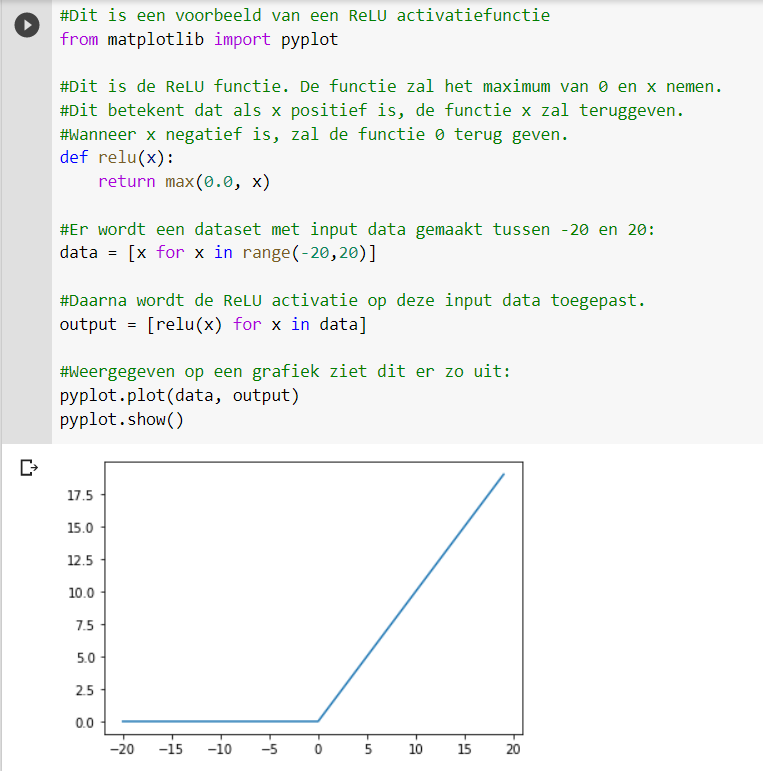
\includegraphics[width=\textwidth]{ReLU.PNG}
    \caption{\label{ReLU}De ReLU activatiefunctie \autocite{Brownlee2021}.}
\end{figure}
\FloatBarrier


\subsubsection{Sigmoïde}
\label{sec:sigmoide}

De sigmoïde activatiefunctie zorgt ervoor dat elke input een output tussen 0 en 1 wordt. Ook hier kan de grafiek dus nooit in het negatieve gaan. Hoe hoger de input, hoe dichter bij 1 en omgekeerd. De sigmoïde functie wordt ook gebruikt bij logistische regressie, maar dit wordt niet in deze bachelorproef besproken. \autocite{Brownlee2021} De sigmoïde activatiefunctie gebeurt als volgt:

\begin{figure}[!htbp]
    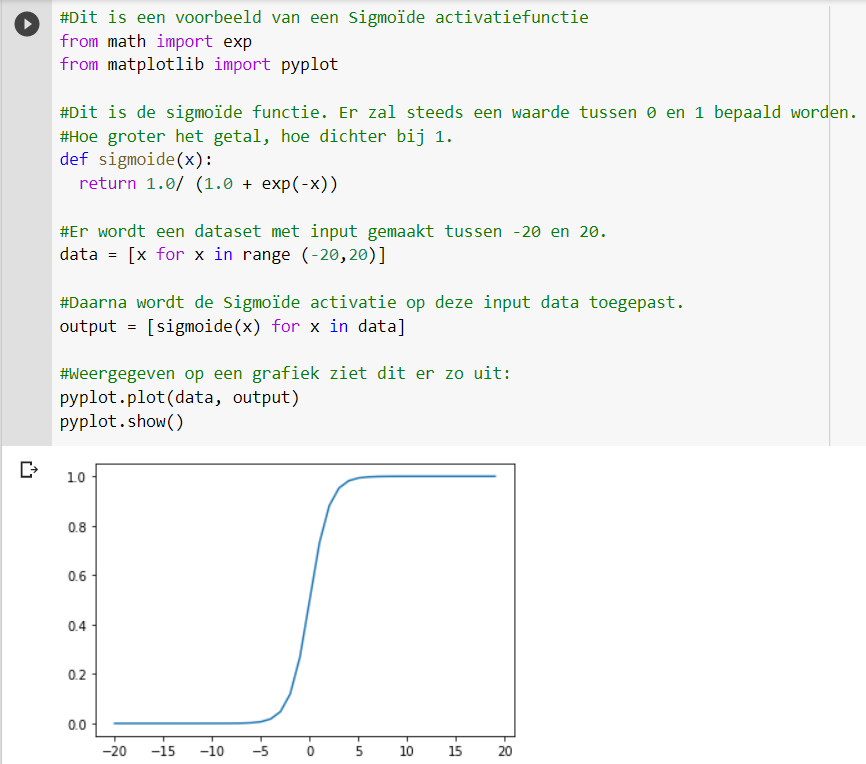
\includegraphics[width=\textwidth]{sigmoide.PNG}
    \caption{\label{sigmoide}De sigmoïde activatiefunctie \autocite{Brownlee2021}.}
\end{figure}
\FloatBarrier


\subsubsection{Tanh}
\label{sec:tanh}

De Tanh activatiefunctie lijkt een beetje op de sigmoïde activatiefunctie in die zin dat ze allebei die S-vorm vertonen. Het verschil tussen de sigmoïde activatiefunctie en de tanh activatiefunctie is dat de tanh activatiefunctie de input omzet in waarden tussen -1 en 1. Waardoor dit de enige activatiefunctie is waarbij de output negatief kan zijn. Hoe groter de input, hoe dichter bij 1, hoe kleiner de input, hoe dichter bij -1. \autocite{Brownlee2021}

\begin{figure}[!htbp]
    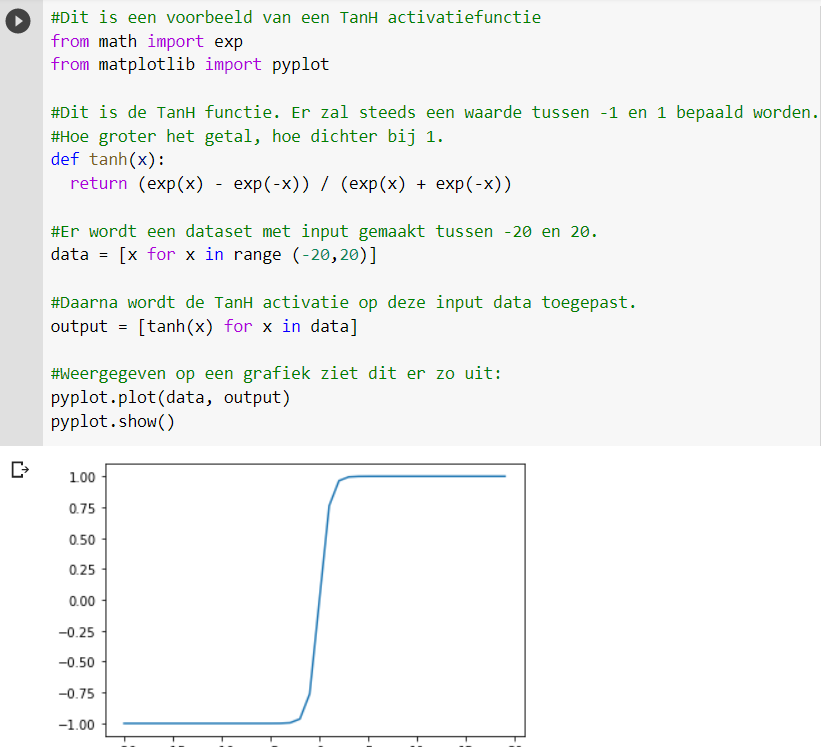
\includegraphics[width=\textwidth]{tanh.PNG}
    \caption{\label{tanh}De Tanh activatiefunctie \autocite{Brownlee2021}.}
\end{figure}
\FloatBarrier


\section{Natural Language Processing}
\label{sec:NLP}

In dit hoofdstuk wordt besproken wat NLP of Natural Language Processing juist is. Daarnaast worden enkele interessante technieken besproken die in het onderzoek naar NLP zeker toegepast zullen worden. 

\subsection{Wat is NLP?}
\label{sec:WatisNLP}
NLP staat voor Natural Language Processing en is het hoofdonderwerp van deze bachelorproef. Natural Language processing is het deelveld van artificiële intelligentie dat zich bezighoudt met taal. Deze term geeft machines of computers de mogelijkheid om tekst of spraak te herkennen. NLP maakt gebruik van machine learning en deep learning om taal te herkennen. Deze onderwerpen werden hiervoor al besproken. De NLP technologie stelt een machine niet enkel in staat om tekst te herkennen, maar ook om deze te ‘begrijpen’. Zo zijn de vertaaltools begonnen. NLP houdt niet enkel het herkennen van teksten in, maar ook het vertalen en begrijpen van teksten. Enkele voorbeelden hiervan zijn Google Translate en DeepL. NLP komt niet enkel voor in vertaaltools, maar ook bij digitale assistenten of chatbots. \autocite{IBM2020}

Het analyseren van teksten, zinnen of uitgesproken woorden is niet gemakkelijk. De menselijke taal is heel complex. Mensen drukken zich vaak op heel veel verschillende manieren uit, en het is aan de machine om dit te interpreteren. Naast honderden talen, heeft elke taal nog vele dialecten. Daarnaast heeft elke taal zijn eigen grammaticaregels, termen en syntaxisregels.
Op vlak van spraak gestuurde NLP, verspreekt een persoon zich al snel, of kan deze met een dialect praten. \autocite{sas2020}

Natural Language Processing heeft veel technieken om de menselijke taal te interpreteren. NLP breekt de volledige teksten op in stukjes. Daarna probeert NLP de relaties tussen deze stukjes te analyseren en begrijpen. Enkele belangrijke taken van NLP zijn tokenization and parsing, language detection en lemmatization/stemming. \autocite{sas2020}

\subsubsection{Language detection}
\label{sec:Languagedetection}

Wanneer een tekst onderzocht wordt, moet de machine eerst bepalen in welke taal deze tekst staat. Wanneer er meerdere talen in 1 tekst staan, worden er meerdere classificatie modellen gemaakt, 1 per taal. In figuur 2.5 wordt dit getest met de zin ‘vandaag is een prachtige dag' in verschillende talen. 

\begin{figure}[!htbp]
    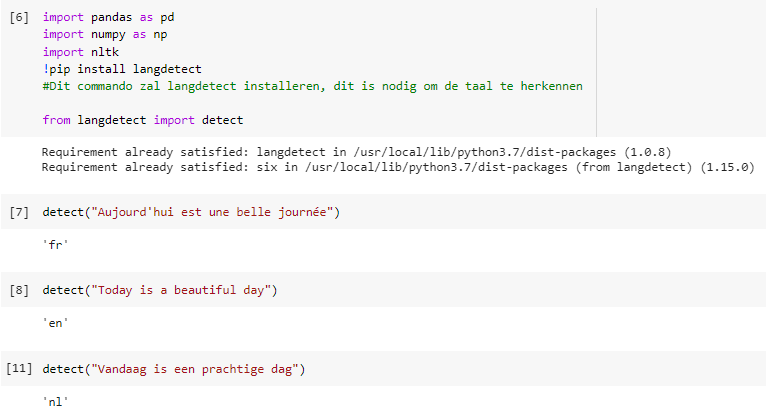
\includegraphics[width=\textwidth]{langdetect.PNG}
    \caption{\label{languagedetection}Language Detection \autocite{sas2020}.}
\end{figure}
\FloatBarrier

\subsubsection{Tokenization and parsing}
\label{sec:Tokenization}

Tokenization is een NLP techniek waarbij een string of zin in kleinere tokens opgedeeld wordt. Tokenization is belangrijk omdat in NLP de tekst geanalyseerd wordt op tokens. 

\begin{figure}[!htbp]
    \includegraphics[width=\textwidth]{tokenization.PNG}
    \caption{\label{tokenization}Tokenization and parsing \autocite{sas2020}.}
\end{figure}
\FloatBarrier

\subsubsection{Stemming and lemmatization}
\label{sec:stemming}

Stemming en lemmatization zijn twee NLP technieken die lijken op elkaar, maar toch verschillen op bepaalde vlakken. Het zijn beiden tekst normalisatie technieken. Stemming en lemmatization baseren zich allebei op het feit dat woorden afgestamd zijn van een ander woord. Zo hebben we bijvoorbeeld het werkwoord ‘spelen’. Van het werkwoord spelen kan gezegd worden dat het afstamt van speel. ‘Speelt’ en ‘speelde’ stammen ook af van de stam ‘speel’. Het verschil tussen stemming en lemmatization is dat lemmatization rekening houdt met de context van het woord. \autocite{sas2020}

\begin{figure}[!htbp]
    \includegraphics[width=\textwidth]{stemming.png}
    \caption{\label{stemming}Stemming and lemmatization \autocite{sas2020}.}
\end{figure}
\FloatBarrier

NLP wordt vaak gebruikt in het alledaagse leven. Alexa en Siri zijn heel gekende voorbeelden, maar deze techniek wordt ook in veel andere toepassingen gebruikt, zoals bij spam filtering. 

\subsection{Text Analytics}
\label{sec:textanalytics}

Text analytics of text mining is een techniek die veel wordt teruggevonden in Natural Language Processing. Dankzij deze techniek wordt tekst zonder structuur gemakkelijk omgezet in een gestructureerde dataset. \autocite{Linguamatics2021} Deze dataset is nodig om het model te kunnen trainen, zoals uitgelegd in Hoofdstuk 2: Datasets en gegevensvergaring.
Text mining is enorm belangrijk. In het dagelijkse leven komt iedereen in aanraking met tekst, denk maar aan e-mails, digitale assistenten, chatbots of posten op sociale media. In deze bachelorproef worden volzinnen uit recensies geanalyseerd op een positieve of negatieve connotatie. Text mining zal hier aan te pas komen op deze ongestructureerde volzinnen in een gestructureerde dataset om te vormen. Tijdens dit proces zal NLP aan de hand van machine learning toegepast worden. 

\section{Sentiment Analysis}
\label{sec:sentimentanalysis}

In dit hoofdstuk wordt het begrip Sentiment Analysis besproken. Ten tweede wordt ook kort ingegaan op wat gevoelswaarden juist zijn. Verder wordt ook de problematiek van deze bachelorproef uitgelegd: waarom is het nu zo moeilijk om sentiment uit een tekst te halen?  

\subsection{Wat is Sentiment Analysis?}
\label{sec:watissentimentanalysis}

Sentiment Analysis is het onderzoek dat in deze bachelorproef wordt gevoerd. Er wordt een sentiment analyse uitgevoerd op recensies. Sentiment analyse is een Natural Language Processing (NLP) techniek die gebruikt wordt om te onderzoeken of een tekst een positieve, neutrale of negatieve connotatie heeft. Klanten drukken vaak hun gevoelens uit in de vorm van recensies. Het is voor bedrijven essentieel om op deze gevoelens in te spelen. Met sentiment analysis kan een bedrijf de feedback van de klant analyseren en begrijpen. \autocite{MonkeyLearn2021}
 
Dankzij Sentiment Analysis kan een bedrijf te weten komen wat er in het hoofd van hun klanten omgaat. Sentiment Analysis kan niet enkel de reviews van de klant analyseren als positief/negatief, maar kan dit ook koppelen aan een bepaald product. Zo weet het bedrijf van welk product de klanten het meest tevreden zijn. \autocite{MonkeyLearn2021}

Er zijn verschillende soorten sentiment analysis, zoals emotiedetectie, multilingual sentiment analysis en aspect-based sentiment analysis. 

Emotiedetectie is een soort sentiment analysis die zich bezig houdt met het achterhalen van gevoelens uit teksten. Deze gevoelens kunnen boosheid, blijheid, verdriet en veel meer uitdrukken. \autocite{MonkeyLearn2021}

Aspect-based sentiment analysis is de techniek die toegepast zal worden in het onderzoek van deze bachelorproef. Bij deze techniek komt een bedrijf te weten over welke features of producten de klant zich positief of negatief uitdrukt. \autocite{MonkeyLearn2021}

Aspect-based sentiment analysis analyseert ten eerste de sentimenten van de tekst, en ten tweede ook de aspecten (features of producten) waarover de gevoelens gaan.
 
Multilingual sentiment analysis is hetzelfde als sentiment analysis, maar met de gedachte dat een review in de eigen taal moet geanalyseerd worden, om geen context of connotatie te verliezen. \autocite{MonkeyLearn2021}

\subsection{Sentiment Analysis en Algoritmen}
\label{sec:sentimentanalysisenalgoritmen}

Bij het implementeren van het sentiment analysis model, zijn er drie soorten algoritmes die men kan gebruiken. (MonkeyLearn, 2021)

\subsubsection{Rule based}
\label{rule based}

Rule based algoritmen voeren de analyse uit op basis van een set regels. Deze regels kunnen ook bestaan uit NLP technieken zoals tokenization. Algoritmen gebaseerd op regels bepalen twee lijsten. Een lijst met positieve woorden zoals ‘goed’, ‘mooi’, ‘prachtig’ en ‘super’, en een lijst met negatieve woorden zoals ‘slecht’, ‘ontevreden’,  en  ‘lelijk’. Daarna telt het algoritme het aantal woorden uit deze lijst dat voorkomt in de gegeven tekst of review. Als er meer positieve woorden geteld zijn dan negatieve, dan wordt de tekst gezien als positief. Dit is dus omgekeerd ook het geval. \autocite{MonkeyLearn2021}

\subsubsection{Automatic}
\label{automatic}

Bij dit algoritme gebruikt men machine learning technieken, waarbij de data getraind wordt. Wanneer we dan een tekst of review in dit algoritme steken, zal het algoritme daar een negatieve, neutrale of positieve connotatie aan toekennen. Dit gebeurt aan de hand van deep learning. \autocite{MonkeyLearn2021}

\subsubsection{Hybrid}
\label{hybrid}

Bij hybrid algoritmen, maakt het algoritme gebruik van zowel rule-based als automatic algoritmen. \autocite{MonkeyLearn2021}

\subsection{Wat zijn gevoelswaarden?}
\label{gevoelswaarden}

In de context van deze bachelorproef kunnen recensies gevoelswaarden bevatten. Ten eerste zijn er positieve gevoelswaarden. Dit gaat over recensies die lovende kritiek geven over het product of het product aanraden. Enkele voorbeelden van positieve recensies: 

\begin{itemize}
    \item “Ik gebruik de laptop veel onderweg in de trein. Super makkelijk om mee te nemen. Hij start snel op en is perfect voor mijn werk.”
    \item “Zoals altijd super een superspannend boek van een geweldige schrijver. Heerlijk!”
\end{itemize}

Echter kunnen recensies ook negatief zijn. Enkele voorbeelden van negatieve recensies:

\begin{itemize}
    \item “Deze jas heeft geen ritssluiting, waardoor de kans bestaat dat er regen doorkomt. Dit is niet wat ik verwacht had.”
    \item “Teleurstellend. Het telefoonhoesje was beschadigd bij ontvangst.”
\end{itemize}

\subsection{Waarom is het moeilijk voor AI's om sentiment te analyseren?}
\label{moeilijksentimentanalyseren}

\subsubsection{Subjectiviteit}
\label{subjectiviteit}

Gevoelens zijn subjectief. Er zijn talloze manieren waarop iemand zich kan uitdrukken, de één al positiever dan de ander. 

\subsubsection{Context}
\label{context}

De context van bepaalde woorden is ook enorm belangrijk. Een voorbeeld: “De auto was bij aankoop goed beschadigd”. In deze zin zit het woordje ‘goed’, maar dit betekent niet dat de review een positieve connotatie heeft, integendeel. \autocite{MonkeyLearn2021}

\subsubsection{Ironie en sarcasme}
\label{ironiesarcasme}

Ironie en sarcasme zijn twee zaken die een machine moeilijk kan herkennen. Wanneer iemand ironie of sarcasme gebruikt, drukt hij zijn negatieve gevoelens over een bepaald aspect uit met positieve woorden. \autocite{MonkeyLearn2021} Een voorbeeld hiervan: “Wauw, dat ging goed!”. Deze zin kan zowel in een positieve context gezien worden, maar kan ook sarcastisch opgenomen worden. 

\subsubsection{Vergelijkingen}
\label{vergelijkingen}

Ook vergelijkingen kunnen door elkaar gebruikt worden. We kunnen ‘beter dan’ gebruiken in verschillende contexten. 

\begin{itemize}
    \item “Deze smartphone is beter dan de vorige versie.”
\end{itemize}

Deze review heeft duidelijk een positieve context, maar we kunnen ook deze review analyseren:


\begin{itemize}
    \item “Deze smartphone is trager dan gewoonlijk, maar het is beter dan niets.”
\end{itemize}

In deze context, is ‘beter dan’ helemaal niet positief. Dit toont ook aan waarom het voor artificiële intelligentie zo moeilijk is om een sentiment uit een zin te halen. 


\section{Gevoelswaarden detecteren in teksten}
\label{gevoelswaardendetecteren}

Sentiment of gevoelswaarden kunnen op verschillende manieren gedetecteerd worden in teksten. Daarom worden in dit hoofdstuk enkele manieren besproken die in de methodologie zullen toegepast worden. 

\subsection{SaaS (Software as a Service)}
\label{saas}

Wanneer een model voor sentiment analysis zou geschreven moeten worden, dan zou er een team aan programmeurs en een grote som geld nodig zijn. Daarom is het interessant om SaaS-tools te gebruiken. SaaS platforms bieden software als een service aan. Dit betekent dat de gebruiker deze software via het internet kan gebruiken, maar deze niet op zijn computer kan downloaden. \autocite{Marketing2021} Deze techniek wordt zeker gebruikt in het methodologie-gedeelte. De software-platforms hieronder zijn voorbeelden van SaaS. 

\subsubsection{MonkeyLearn}
\label{monkeylearn}

Monkeylearn is een platform dat services aanbiedt om tekst te analyseren aan de hand van machine learning en sentiment analysis. Het voorziet een grafische user interface om zelf reviews in te geven en deze te trainen. \autocite{Maguire2021} Het platform van MonkeyLearn zal getest en gebruikt worden tijdens het onderzoek.

\subsubsection{Text Analytics API}
\label{textanalytics}

Text Analytics API is een service die NLP aan de gebruiker aanbiedt. Technieken zoals sentiment analysis en opinion mining kunnen worden uitgevoerd aan de hand van deze service. Deze API maakt deel uit van Azure Cognitive Services. \autocite{Microsoft2020} Deze Tekst Analytics API kan gebruikt worden in Visual Studio Code aan de hand van REST API. Ook deze service zal getest en gebruikt worden tijdens het onderzoek.

Naast SaaS-tools, kan men ook zelf een dataset zoeken en deze trainen. Dit wordt verder besproken in het volgende hoofdstuk.

\section{De Datasets}
\label{datasets} 

Zoals hiervoor aangehaald, is het natuurlijk ook mogelijk om zelf een dataset te gebruiken en deze te trainen. In dit onderzoek worden er twee datasets gebruikt.

\subsection{Amazon Dataset}
\label{amazon}

De eerste dataset is de \textbf{Amazon dataset}. Deze dataset bevat reviews van de producten die op de populaire website Amazon verkocht worden. Deze dataset bevat meer dan 233 miljoen reviews, daardoor zal niet deze volledige dataset gebruikt worden. De reviews van deze dataset werden verzameld tussen 1996 en 2018. \autocite{Ni2019} Een voorbeeld van hoe 1 review er uit ziet in de dataset kan hieronder gevonden worden: 
  
\begin{table}[]
    \begin{tabular}{@{}|l|l|@{}}
        \toprule
        \textbf{Attribute} & \textbf{Content}                                                                                                                                                                                                                                                                                        \\ \midrule
        reviewerID         & A2SUAM1J3GNN3B                                                                                                                                                                                                                                                                                          \\
        asin               & 0000013714                                                                                                                                                                                                                                                                                              \\
        reviewerName       & J. McDonald                                                                                                                                                                                                                                                                                             \\
        helpful            & {[}2,3{]}                                                                                                                                                                                                                                                                                               \\
        reviewText         & \begin{tabular}[c]{@{}l@{}}I bought this for my husband who plays the piano. \\ He is having a wonderful time playing these old hymns. \\ The music is at times hard to read because we think the book\\  was published for singing from more than playing from. \\ Great purchase though!\end{tabular} \\
        overall            & 5.0                                                                                                                                                                                                                                                                                                     \\
        summary            & Heavenly Highway Hymns                                                                                                                                                                                                                                                                                  \\
        unixReviewTime     & 1251800000                                                                                                                                                                                                                                                                                              \\
        reviewTime         & 09 13, 2009                                                                                                                                                                                                                                                                                             \\ \bottomrule
    \end{tabular}
    \caption{Attributen van de Amazon Dataset}
    \label{tab:amazondataset}
\end{table}

\subsection{Twitter US Airline Sentiment Dataset}
\label{twitter}

De tweede dataset is de \textbf{Twitter US Airline Sentiment dataset}. Deze dataset bevat reviews in de vorm van tweets. Deze reviews gaan over de bekendste US vluchtmaatschappijen.\autocite{Kaggle2020} Een voorbeeld van hoe 1 review er uit ziet in de database kan hieronder gevonden worden:
\begin{table}[]
    \begin{tabular}{@{}|l|l|@{}}
        \toprule
        \textbf{Attribute}             & \textbf{Content}            \\ \midrule
        tweet\_id                      & 570306133677760513          \\
        airline\_sentiment             & neutral                     \\
        airline\_sentiment\_confidence & 0.3486                      \\
        negativereason                 & Bad Flight                  \\
        negativereason\_confidence     & 0.7033                      \\
        airline                        & Virgin America              \\
        airline\_sentiment\_gold       & NaN                         \\
        name                           & jnardino                    \\
        negativereason\_gold           & NaN                         \\
        retweet\_count                 & 0                           \\
        text                           & @VirginAmerica, Thanks!     \\
        tweet\_coord                   & NaN                         \\
        tweet\_created                 & 2015-02-24 11:35:52-0800    \\
        tweet\_location                & San Francisco CA            \\
        user\_timezone                 & Pacific Time (US \& Canada) \\ \bottomrule
    \end{tabular}
    \caption{Attributen van de Twitter US Airline Sentiment Dataset}
    \label{tab:twitterdataset}
\end{table}


%%=============================================================================
%% Methodologie
%%=============================================================================

\chapter{\IfLanguageName{dutch}{Methodologie}{Methodology}}
\label{ch:methodologie}

%% TODO: Hoe ben je te werk gegaan? Verdeel je onderzoek in grote fasen, en
%% licht in elke fase toe welke stappen je gevolgd hebt. Verantwoord waarom je
%% op deze manier te werk gegaan bent. Je moet kunnen aantonen dat je de best
%% mogelijke manier toegepast hebt om een antwoord te vinden op de
%% onderzoeksvraag.

In dit gedeelte van de bachelorproef wordt onderzocht of AI klaar is om Sentiment Analysis toe te passen in het bedrijfsleven. Er zullen een aantal mogelijkheden worden getest om te zien welke tool het nauwkeurigste is. Zoals eerder vermeld, zal Sentiment Analysis klaar zijn om te gebruiken in het bedrijfsleven bij een succespercentage van 80 \%. 

De eerste tool die getest wordt is de Microsoft Azure Text Analytics API. 

\section{Microsoft Azure Text Analytics API}

\subsection{Achtergrond informatie}
\label{achtergrondinformatieazure}
Zoals eerder besproken, biedt Microsoft Azure SaaS-tools aan in de vorm van software. De Text Analytics API biedt dus ook NLP features aan voor text mining, text analysis, sentiment analysis, opinion mining,... \autocite{Microsoft2020} Deze API maakt deel uit van de Azure Cognitive Services. Deze biedt een volledig aanbod aan machine learning en AI algoritmes. Om deze services te gebruiken , moet de gebruiker wel een account aanmaken. \autocite{Microsoft2020}

Om deze Microsoft Text Analytics API te implementeren zal er gebruik gemaakt worden van Microsoft Visual Studio. Microsoft Visual Studio is een IDE (Integrated Development Environment) en wordt gebruikt om applicaties, websites en software te ontwikkelen voor Windows. Voor deze bachelorproef wordt de code in Microsoft Visual Studio geschreven, met name in de programmeertaal C\#. 

\subsection{Aanpak}
\label{aanpakazure}
\textbf{Stap 1}: De Text Analytics Resource

Om te beginnen moet er een Text Analytics Resource gemaakt worden in Azure zoals te zien op figuur 3.1. Een Text Analytics Resource is een service waardoor de gebruiker teksten kan analyseren zonder daarvoor de AI te moeten trainen. \autocite{Microsoft2020}

\begin{figure}[!htbp]
    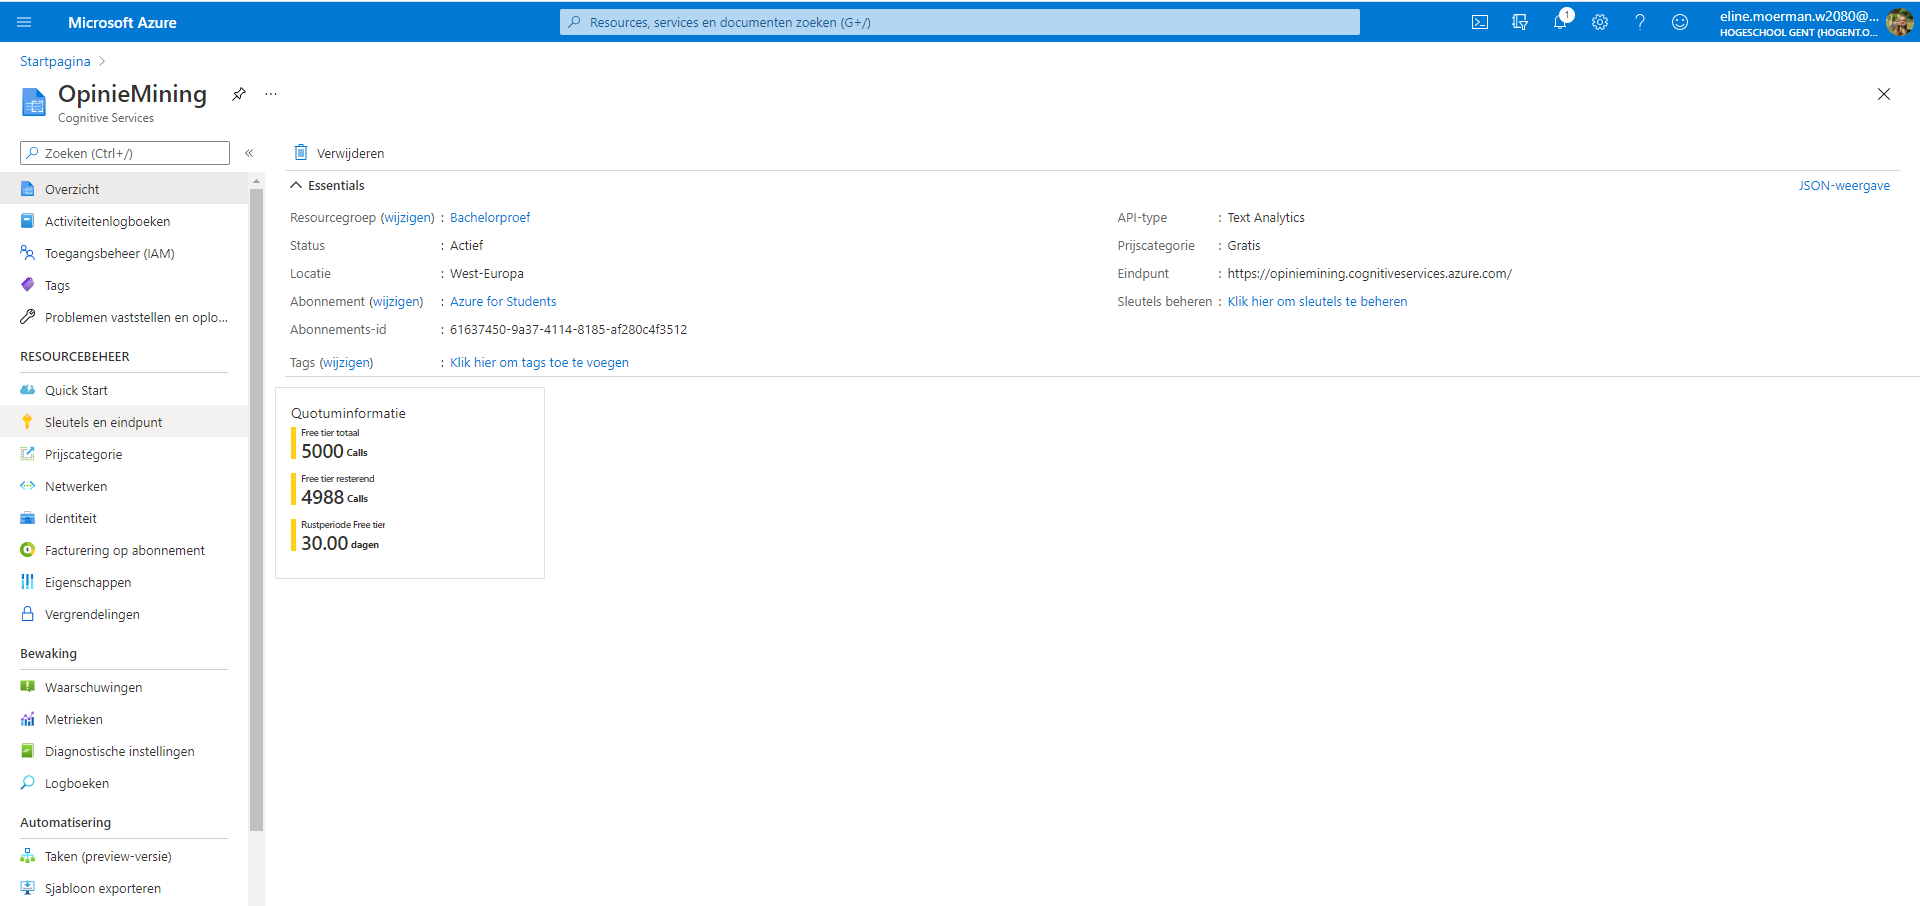
\includegraphics[width=\textwidth]{AzureResource.PNG}
    \caption{\label{azureresource}De Azure Text Analytics Resource \autocite{Microsoft2021}.}
\end{figure}
\FloatBarrier

Eenmaal dat de service aangemaakt is, genereert Azure een sleutel en een endpoint. Deze zullen gebruikt worden in Visual Studio om de Azure service te kunnen gebruiken. De key en endpoint zijn nodig zodat niemand anders van deze service kan gebruik maken. 

\textbf{Stap 2}: Een project opzetten in Visual Studio en de juiste packages installeren

Wanneer Visual Studio opgestart wordt, vraagt de applicatie om een nieuw project te maken. Hier is de beste keuze een .NET Core console applicatie. Dit zorgt ervoor dat er geen overbodige bestanden worden aangemaakt en dat enkel de klasse Program.cs aangemaakt zal worden. In deze file zal al de code geschreven worden om de datasets te kunnen analyseren. \autocite{Microsoft2020}

Daarna moet er een package geïnstalleerd worden. Een package is herbruikbare code die al door andere developers geschreven is en die de gebruiker kan downloaden in zijn of haar project. \autocite{Microsoft2018} De package die nodig is is Azure.AI.TextAnalytics, zoals te zien op figuur 3.2.

\begin{figure}[!htbp]
    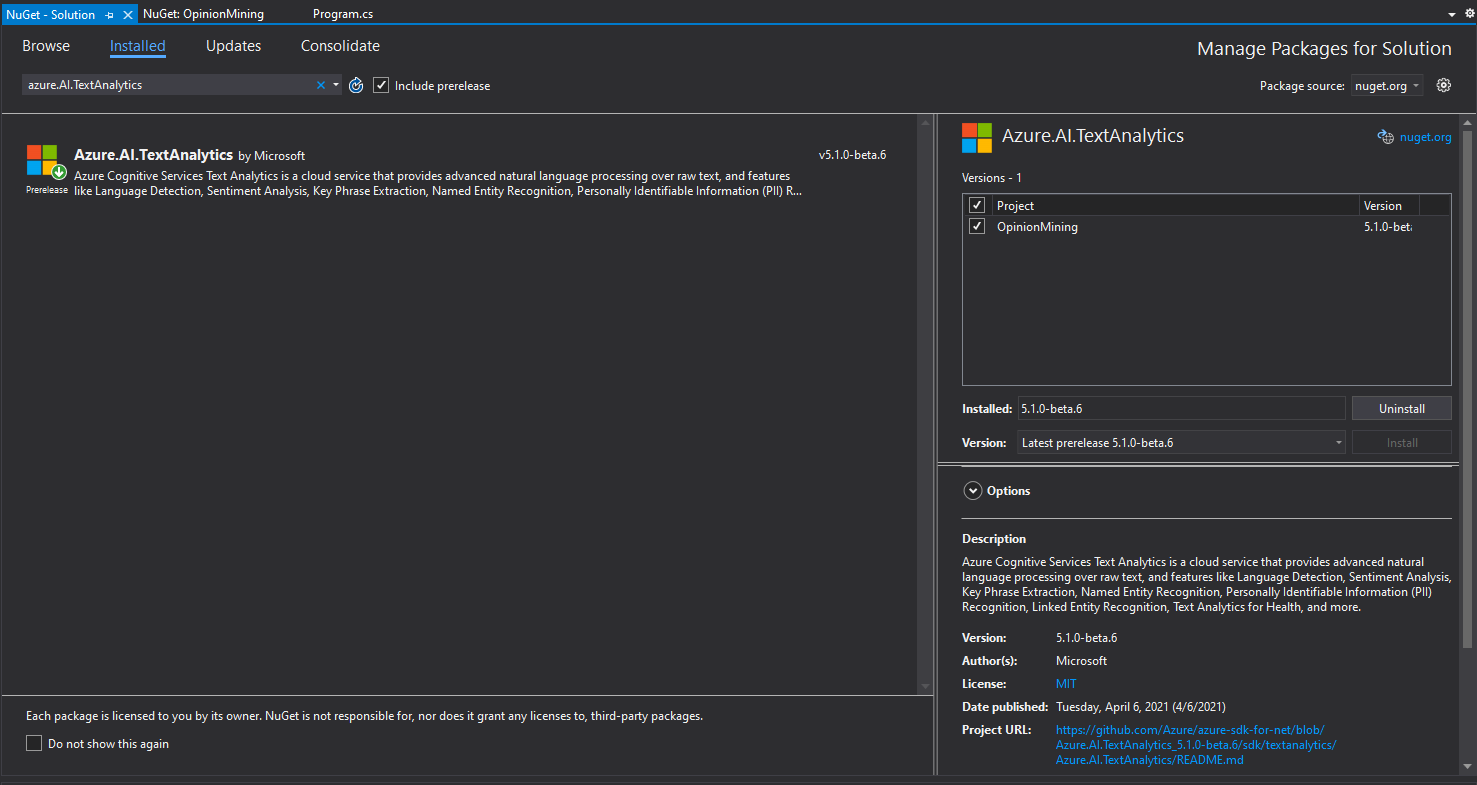
\includegraphics[width=\textwidth]{AzurePackage.PNG}
    \caption{\label{azurepackage}De Azure TextAnalytics Package \autocite{Microsoft2020}.}
\end{figure}
\FloatBarrier


\textbf{Stap 3}: De data omzetten naar het juiste formaat

Om de data uit de datasets te gebruiken, moeten we deze kunnen toevoegen in Visual Studio. Allereerst wordt er een nieuwe klasse 'Data' aangemaakt. Hier zal alle data opgeslagen worden zodat deze later kan gebruikt worden. Daarna wordt er een een nieuw Google Colab document aangemaakt. Een Google Colab document is een tool waar de gebruiker code in Python kan schrijven. Dit gebeurt allemaal online, er moet geen software gedownload worden om deze tool te kunnen gebruiken. 

\textbf{Stap 4}: De juiste code schrijven om zinnen te kunnen analyseren

Met behulp van de Azure Text Analytics documentatie, kan de code in enkele methoden geschreven worden. Alle code wordt geschreven in de klasse Program.cs. 

\subsection{Amazon Dataset}
\label{amazondatasetazure}

\subsubsection{Data omzetten}
\label{amazondatasetomzettenazure}
Wanneer de Amazon dataset van het internet gehaald wordt, krijgt de gebruiker twee bz2 bestanden. Deze moeten natuurlijk omgezet worden zodat de data in Visual Studio geanalyseerd kan worden. Het is handig om de bestanden op Google Drive op te slaan aangezien men hier heel gemakkelijk vanuit een Google Colab document aankan. In figuur 3.3 wordt dit proces getoond. Om te beginnen, worden de juiste imports toegevoegd om data te kunnen analyseren. In dit bestand maken we gebruik van pandas, numpy en bz2. Daarna wordt er toegang tot Google Drive gemaakt. In een laatste stap worden de bestanden vanop Google Drive uitgelezen

\begin{figure}[!htbp]
    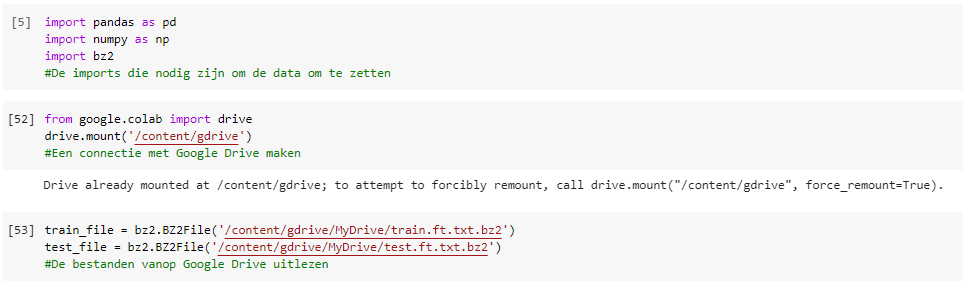
\includegraphics[width=\textwidth]{Stap1Omzetten.PNG}
    \caption{\label{stap1amazon}De bestanden worden opgehaald uit Google Drive.}
\end{figure}
\FloatBarrier

Daarna (figuur 3.4) wordt de data omgevormd tot bruikbare zinnen. Om te beginnen wordt de data via de functie readlines() omgezet naar een lijst van items waar elke lijn een object vormt. In het tweede blokje code wordt aangegeven hoe een review van de dataset er uitziet. Men kan zien dat er voor elke zin nog een b staat. Deze b moet weggefiltert worden, zodat de data naar tekst omgevormd wordt. 

Eenmaal dit gebeurd is, kan men in het vierde blokje code zien dat de b weg is.

\begin{figure}[!htbp]
    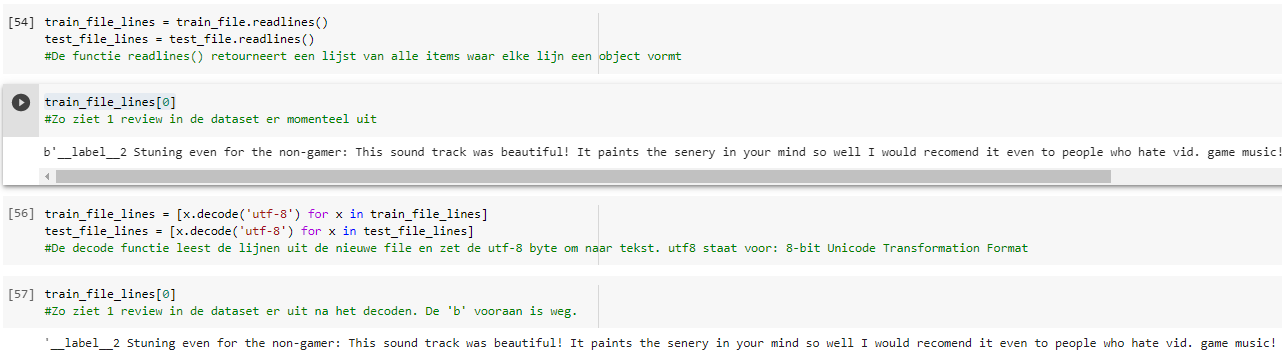
\includegraphics[width=\textwidth]{Stap2Omzetten.PNG}
    \caption{\label{stap2amazon}De data wordt omgezet naar tekst.}
\end{figure}
\FloatBarrier

Echter is dit nog niet genoeg om met deze data verder te werken. Vooraan elke zin staat ook nog een label. Dit label representeert een positieve of negatieve connotatie van de zin. Daarom worden de labels en de tekst opgeplitst in twee datasets, zoals te zien op figuur 3.5. De eerste dataset noemt train\_labels: Deze bevat de sentimenten die bij elke zin horen. Label1 wordt omgezet naar 0, label2 wordt omgezet naar 1. 1 representeert een positieve context, 0 een negatieve context. De tweede dataset heeft als naam train\_sentences: deze dataset bevat de eigenlijke zinnen die we door het programma in Visual Studio zullen laten lopen. In codeblokje twee staat een voorbeeld van hoe een zin er nu uit ziet, in codeblokje 3 staat een voorbeeld van hoe een score er nu uit ziet. 

\begin{figure}[!htbp]
    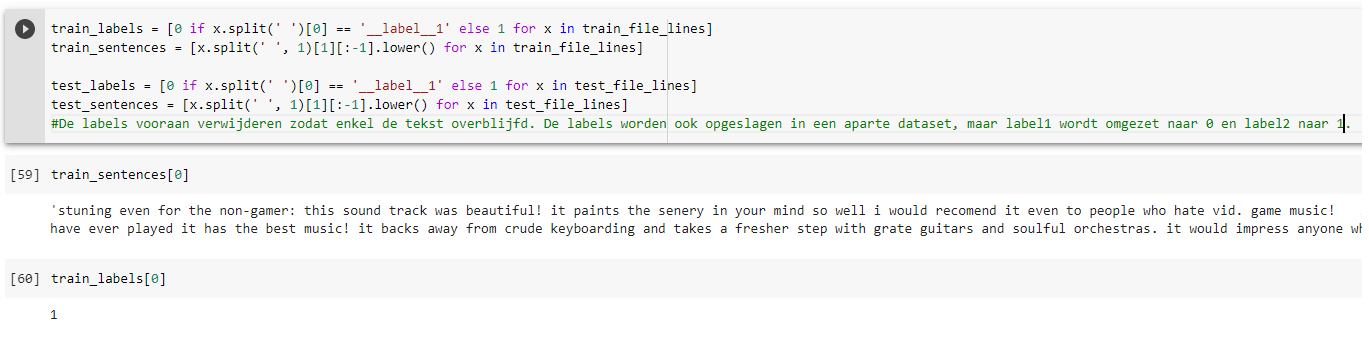
\includegraphics[width=\textwidth]{Stap3Omzetten.PNG}
    \caption{\label{stap3amazon}De data wordt opgeplitst.}
\end{figure}
\FloatBarrier

Verder zijn er veel url's die gebruikt worden in de zinnen. Deze zijn niet nodig om de connotatie van een zin te analyseren. Via onderstaande methode in figuur 3.6 worden de url's uit de tekst gefilterd.

\begin{figure}[!htbp]
    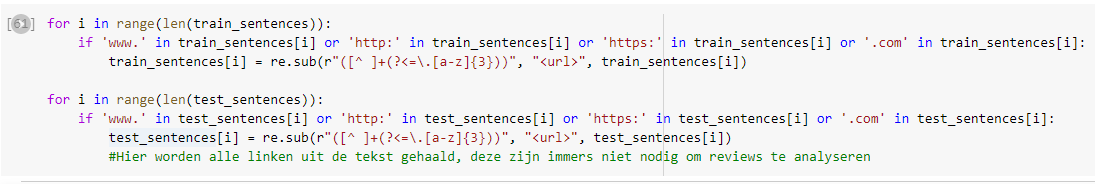
\includegraphics[width=\textwidth]{Stap4Omzetten.PNG}
    \caption{\label{stap4amazon}De url's worden uit de zinnen gehaald.}
\end{figure}
\FloatBarrier

Om te visualiseren hoe de data er momenteel uitziet, worden de zinnen in een dataframe geplaatst. Daarna worden de eerste 100 items getoond via de methode head(100).

\begin{figure}[!htbp]
    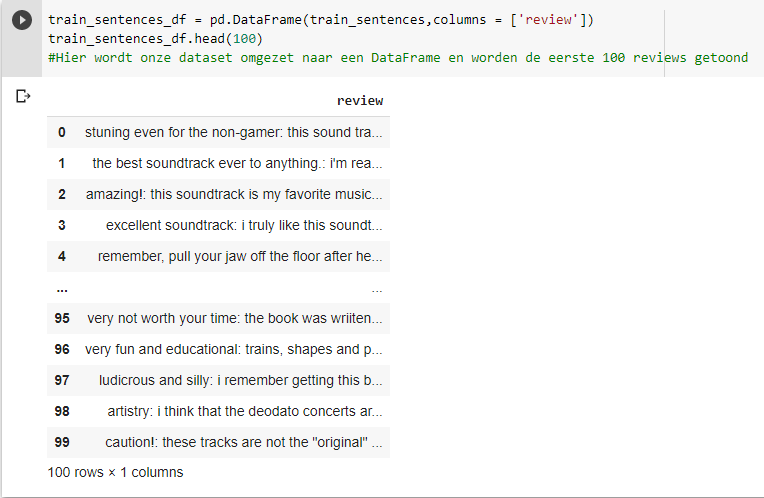
\includegraphics[width=\textwidth]{Stap5Omzetten.PNG}
    \caption{\label{stap5amazon}De data wordt omgezet naar een DataFrame.}
\end{figure}
\FloatBarrier

Zodat de zinnen gemakkelijk in Visual Studio kunnen toegevoegd worden, printen we de eerste 500 zinnen met de methode head(500) en zetten we deze in de vorm Sentences.Add(zin). Zo kan dit gemakkelijk en zonder problemen gekopieerd worden naar Visual Studio.

\begin{figure}[!htbp]
    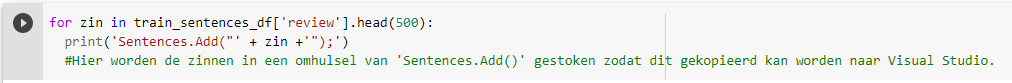
\includegraphics[width=\textwidth]{Stap6Omzetten.PNG}
    \caption{\label{stap6amazon}De zinnen worden in een formaat gestoken dat gemakkelijk in Visual Studio kan gebruikt worden.}
\end{figure}
\FloatBarrier

In figuur 3.9 kan men zien dat de zinnen die hiervoor gegenereerd werden gekopieerd zijn naar de klasse Data. De zinnen worden in een lijst van strings gestoken dat men 'Sentences' noemt. De scores worden in een lijst van ints gestoken, nadat deze omgezet zijn in figuur 3.10.

\begin{figure}[!htbp]
    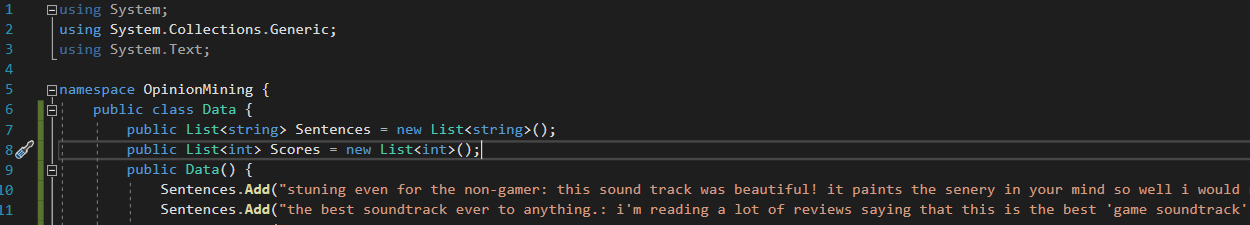
\includegraphics[width=\textwidth]{Stap7Omzetten.PNG}
    \caption{\label{stap7amazon}De zinnen worden toegevoegd in de klasse Data.}
\end{figure}
\FloatBarrier

\begin{figure}[!htbp]
    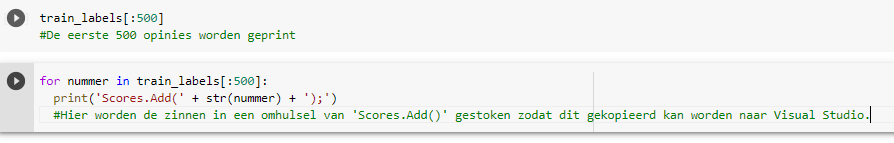
\includegraphics[width=\textwidth]{Stap8Omzetten.PNG}
    \caption{\label{stap8amazon}De scores worden in een formaat gestoken dat gemakkelijk in Visual Studio kan gebruikt worden.}
\end{figure}
\FloatBarrier


\subsubsection{Visual Studio}
\label{amazondatasetvisualstudioazure}
Nu de data-omzetting gebeurd is, beschikt Visual Studio over een lijst van 500 zinnen met bijbehorende score. Een score 0 betekent dat de zin als 'negatief' beschouwd wordt, terwijl een score van 1 een positieve connotatie voorstelt. Om te kijken of de Azure Text Analytics API de zinnen ook werkelijk juist categoriseert, zal er een bepaalde nauwkeurigheid berekend moeten worden. 

Maar om dit te verwezenlijken, moet er eerst een connectie met de Azure Text Analytics resource gemaakt worden. Dit gebeurt aan de hand van de endpoint en de key. Deze worden bovenaan in de klasse Program.cs geplaatst. Alle code zal vanaf nu in deze klasse geschreven worden. 

\begin{figure}[!htbp]
    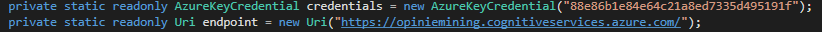
\includegraphics[width=\textwidth]{AzureKeyCredentials.PNG}
    \caption{\label{azurecredentials}De endpoint en key worden bovenaan de klasse geplaatst.}
\end{figure}
\FloatBarrier

Eenmaal de connectie in orde is, kan het onderzoek aan de slag gaan met de Azure Texy Analytics API. Ten eerste zal er getest worden of de Azure resource alle zinnen ook daadwerkelijk herkent als 'Engels'. In sectie 2.3.1 wordt besproken wat Language Detection juist is. Deze techniek zal via een geschreven methode toegepast worden op alle zinnen. Als de getetecteerde zin gelijk is aan 'English', dan zal de nauwkeurigheid (in het codevoorbeeld: accuracy) verhoogd worden met 1. Als alle zinnen juist gezien worden als Engels, wordt er een nauwkeurigheid van 500/500 bereikt. 

\begin{figure}[!htbp]
    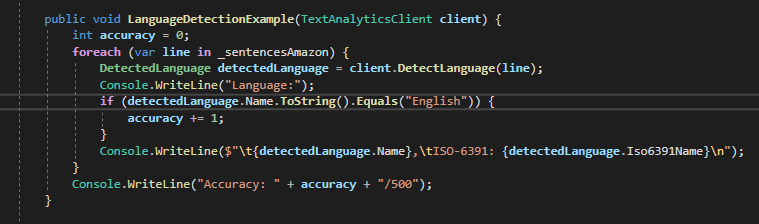
\includegraphics[width=\textwidth]{LanguageDetectionAmazon.PNG}
    \caption{\label{azurelanguagedetectionamazon}Language Detection in Visual Studio.}
\end{figure}
\FloatBarrier

Ten tweede zal er getest worden of de Azure Text Analytics API Sentiment Analysis juist kan toepassen. In sectie 2.4 wordt uitvoerig besproken wat Sentiment Analysis juist is. Via onderstaande methode in figuur 3.13 zal de nauwkeurigheid van de resource getest worden op 500. Bij deze methode is er echter nog wat toelichting nodig. De Azure Text Analytics API kan de zinnen categoriseren als Positief, Neutraal, Negatief en Gemengd. De Amazon dataset bevat enkel de informatie of een zin positief of negatief is. 

Daarom wordt er bij elke zin die juist positief of juist negatief bestempeld wordt, een punt bij de nauwkeurigheid opgeteld. Wanneer de zin als uitkomst Neutraal of Gemengd krijgt, wordt er per stukje tekst gekeken of dit positief of negatief is. Als er meer positieve stukjes zijn dan er negatieve stukjes zijn, wordt deze zin toch bestempeld als positief. Omgekeerd gebeurt hetzelfde voor negatief. 

\begin{figure}[!htbp]
    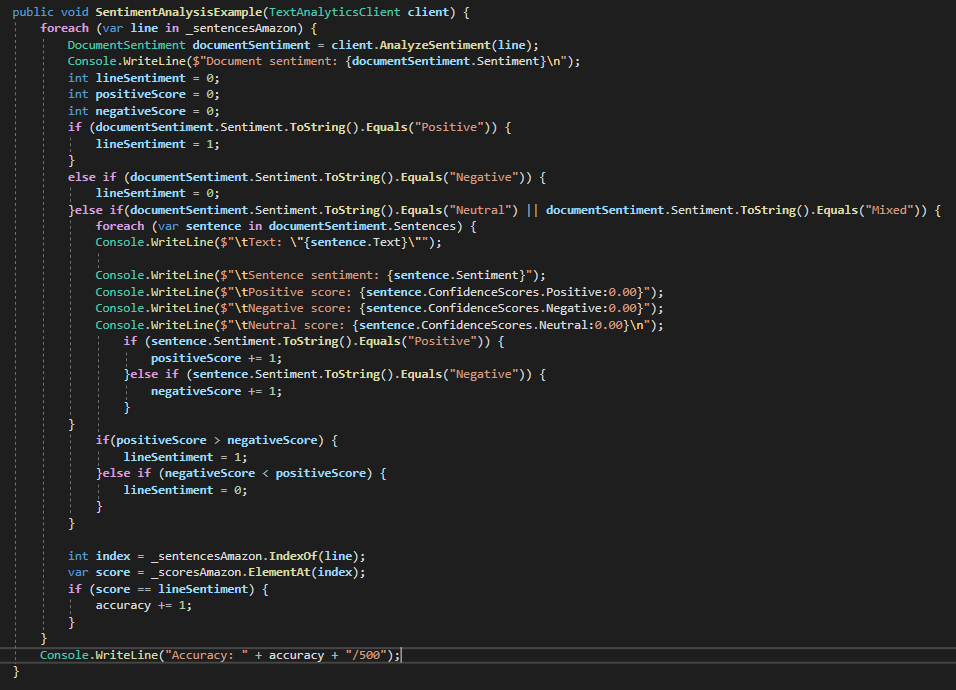
\includegraphics[width=\textwidth]{SentimentAnalysisAmazon.PNG}
    \caption{\label{azuresentimentanalysisamazon}Sentiment Analysis in Visual Studio.}
\end{figure}
\FloatBarrier

\subsubsection{Resultaten}
\label{amazondatasetresultatenazure}
Ten eerste werd er getest of de Azure Text Analytics API alle geselecteerde zinnen uit de dataset categoriseert als 'Engels'. In Figuur 3.14 ziet men dat de nauwkeurigheid 499/500 of 99.8\% is. Er werd 1 zin als 'Spaans' gecategoriseerd.

\begin{figure}[!htbp]
    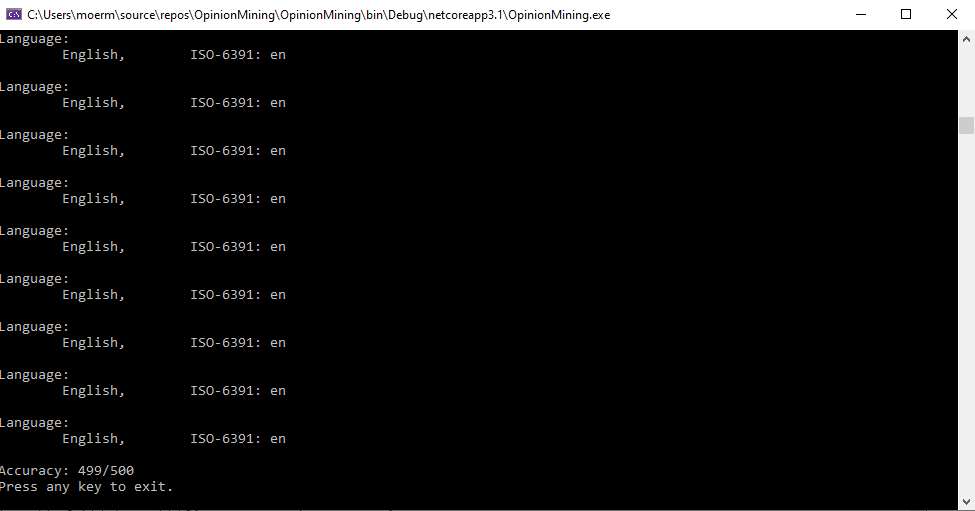
\includegraphics[width=\textwidth]{LanguageDetectionAmazonResult.PNG}
    \caption{\label{azurelanguagedetectionamazonresults}Language Detection voor de Amazon dataset in Visual Studio: Resultaten.}
\end{figure}
\FloatBarrier 

Ten tweede werd er getest of de Azure resource de zinnen uit de dataset juist kan categoriseren als positief of negatief. In figuur 3.15 kunnen de resultaten hiervan gevonden worden. De Azure Text Analytics API heeft 421/500 zinnen juist toegekend. Omgerekend is dit 84.2\%. In sectie 1.3 wordt er bepaald dat als een AI 80\% van de resultaten juist classifieert, dat deze als 'succesvol' kan gezien worden en dus bij bedrijven kan gebruikt worden. Voor deze dataset is dit dus zeker het geval, maar om te bepalen of dit betrouwbaar is, wordt dit ook getest op een tweede dataset, de Twitter Airlines dataset. 

\begin{figure}[!htbp]
    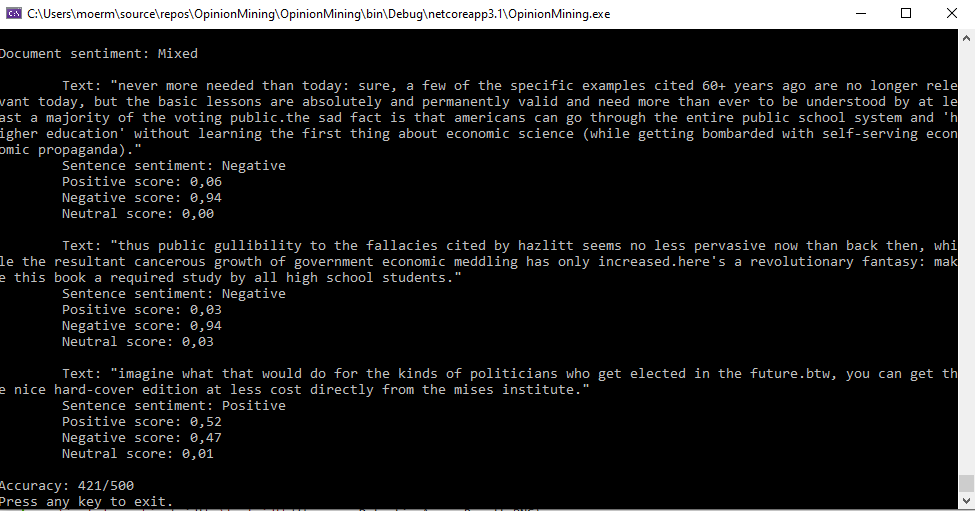
\includegraphics[width=\textwidth]{SentimentAnalysisAmazonResult.PNG}
    \caption{\label{azuresentimentanalysisamazonresults}Sentiment Analysis voor de Amazon dataset in Visual Studio: Resultaten.}
\end{figure}
\FloatBarrier 

\subsection{Twitter Airlines}
\label{twitterdatasetazure}

Ook bij de Twitter Airlines dataset worden dezelfde stappen gevolgd zoals eerder besproken in sectie 3.1.2 Aanpak. Ten eerste zal de data omgezet worden naar het juiste formaat, ten tweede zullen er enkele methodes uitgevoerd worden met deze data en ten slotte zullen de resultaten besproken worden. 

\subsubsection{Data omzetten}
\label{twitterdatasetomzettenazure}
Ook voor deze dataset moet de data omgevormd worden. Deze keer beginnen we met een csv bestand. een csv-bestand bevat 'comma separated values'. Met andere woorden wordt de data gescheiden door een komma. Om te beginnen importeren we juiste imports zoals numpy, pandas en re. Daarna moet er opnieuw verbinding gemaakt worden met Google Drive zodat het juiste csv bestand opgehaald kan worden. 
\begin{figure}[!htbp]
    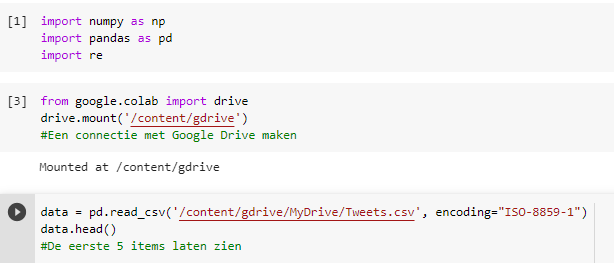
\includegraphics[width=\textwidth]{Stap1Twitter.PNG}
    \caption{\label{azurestap1twitter}Twitter Airline dataset: Imports afhandelen en connectie met Google Drive maken.}
\end{figure}
\FloatBarrier 

Daarna moeten de onnodige kolommen verwijderd worden, en dit zijn er heel wat. Enkel de scores en de zinnen zelf zijn nodig.
\begin{figure}[!htbp]
    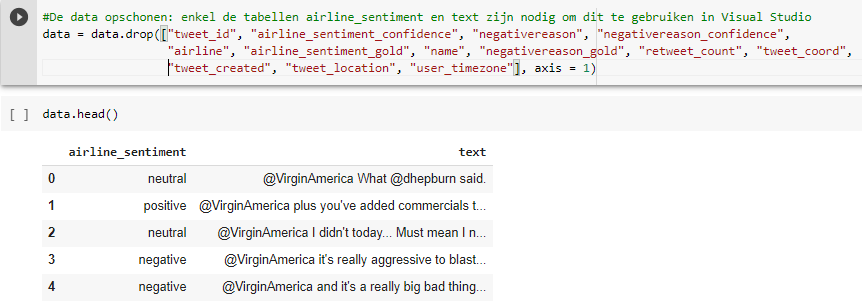
\includegraphics[width=\textwidth]{Stap2Twitter.PNG}
    \caption{\label{azurestap2twitter}Twitter Airline dataset: De onnodige kolommen verwijderen.}
\end{figure}
\FloatBarrier 

Hierna wordt de data opgeplitst. De zinnen worden in een variabele 'zinnen' gestoken, terwijl de scores in een variabele 'sentiment' gestoken worden. 
\begin{figure}[!htbp]
    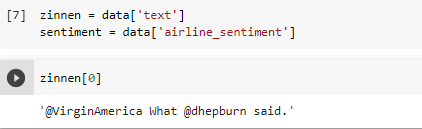
\includegraphics[width=\textwidth]{Stap3Twitter.PNG}
    \caption{\label{azurestap3twitter}Twitter Airline dataset: de score en de zinnen opsplitsen.}
\end{figure}
\FloatBarrier
Ten slotte worden de zinnen, zoals bij de Amazon dataset, in een nieuw formaat afgeprint zodat ze gemakkelijk te kopiëren zijn naar Visual Studio. 
\begin{figure}[!htbp]
    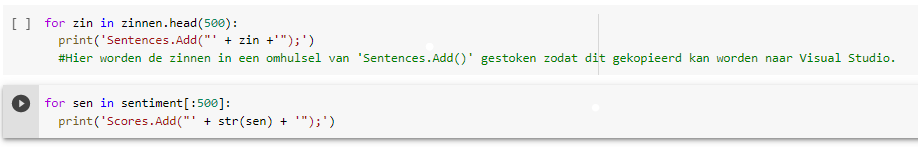
\includegraphics[width=\textwidth]{Stap4Twitter.PNG}
    \caption{\label{azurestap4twitter}Twitter Airline dataset: De zinnen en scores omzetten zodat ze in Visual Studio gebruikt kunnen worden.}
\end{figure}
\FloatBarrier 

\subsubsection{Visual Studio}
\label{twitterdatasetvisualstudioazure}
Voor deze dataset maken we gebruik van dezelfde endpoint en key als bij de vorige dataset, zoals te zien op figuur 3.11. Aan de methode voor gebruik te maken van Language Detection moet er in principe bijna niets aangepast worden. Enkel de dataset verandert. De methode die hier toegepast wordt is ook te zien in figuur 3.12.

Ten tweede wordt ook hier getest of de Azure Text Analytics API de zinnen uit deze dataset kan categoriseren. Hiervoor moet de methode enigzinds aangepast worden aangezien de Twitter dataset wel neutrale connotatie herkent. In deze dataset worden de zinnen gezien als positief, negatief of neutraal. 

\begin{figure}[!htbp]
    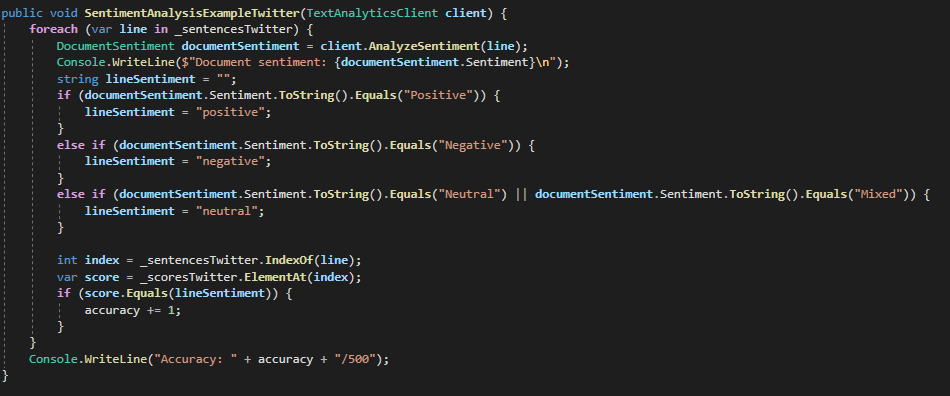
\includegraphics[width=\textwidth]{SentimentAnalysisTwitter.PNG}
    \caption{\label{azuresentimentanalysistwitter}Language Detection voor de Twitter dataset in Visual Studio: Resultaten.}
\end{figure}
\FloatBarrier 


\subsubsection{Resultaten}
\label{twitterdatasetresultatenazure}
Om te beginnen werd hetzelfde als bij de Amazon dataset getest, namelijk of alle zinnen als 'Engels' herkend worden. 
Hier haalt de Azure Text Analytics API een score van 499/500, omgerekend is dit 99.8\%. Één zin werd echter herkend als 'Frans'.

\begin{figure}[!htbp]
    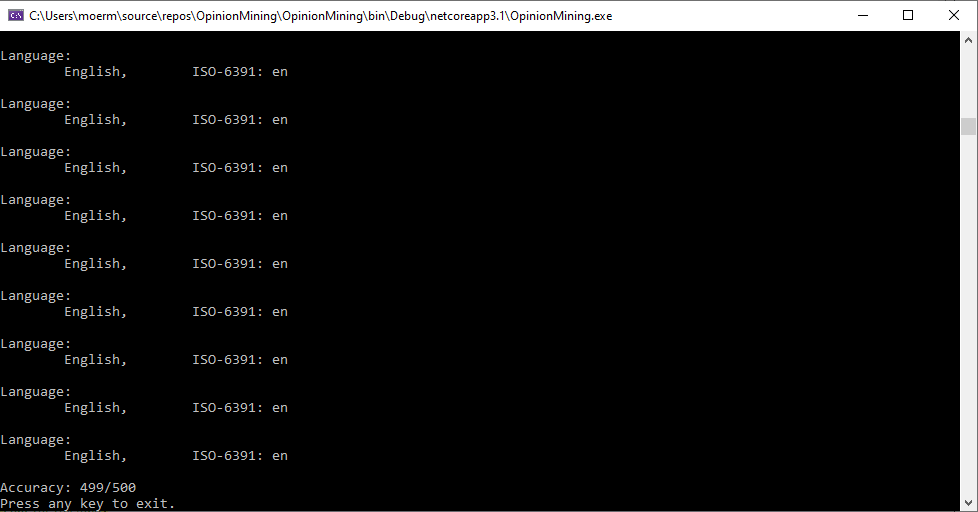
\includegraphics[width=\textwidth]{AccuracyTwitterDatasetAzure.PNG}
    \caption{\label{azurelanguagedetectiontwitterresults}Language Detection voor de Twitter dataset in Visual Studio: Resultaten.}
\end{figure}
\FloatBarrier 

Ten slotte werd er ook getest of Azure de zinnen juist herkent als positief, neutraal of negatief. In figuur xx kunnen de resultaten hiervan terug gevonden worden. Er werd een score van 334/500 behaald door de Azure Text Analytics API. Omgerekend is dit 66.8\%. Dit is minder dan bij de Amazon dataset. Dit kan verklaard worden doordat 'tweets' korter zijn dan reviews, maar ook meer hashtags en apestaartjes bevatten. Verder worden er meer emoji's en tussentaal gebruikt bij tweets dan bij reviews.

\begin{figure}[!htbp]
    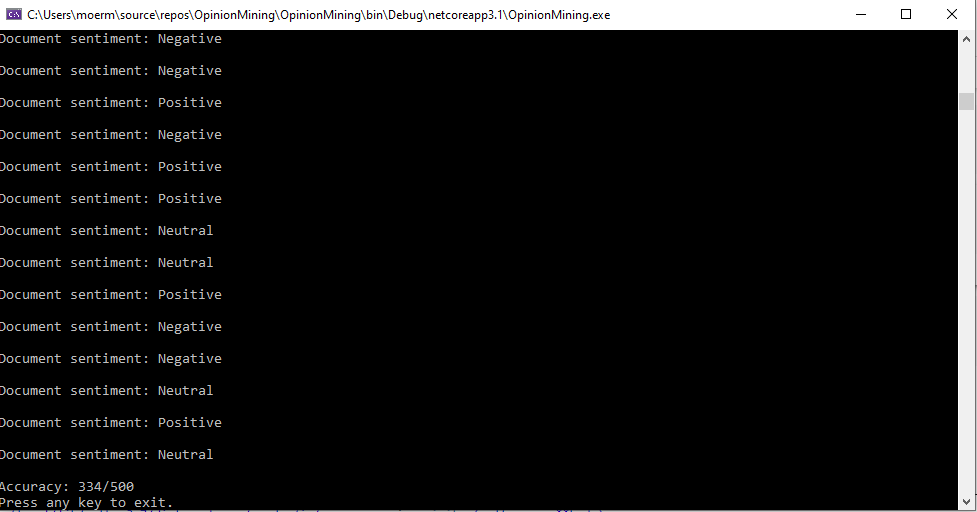
\includegraphics[width=\textwidth]{SentimentAnalysisTwitterResult.PNG}
    \caption{\label{azuresentimentanalysistwitterresults}Sentiment Analysis voor de Twitter dataset in Visual Studio: Resultaten.}
\end{figure}
\FloatBarrier 

\subsection{Conclusie Azure Text Analytics API}
\label{conclusieAzure}
De Azure Analytics API is heel goed voor Language Detection. Bij beide datasets behaalde de tool een score van 99.8\%. Voor Sentiment Analysis waren de resultaten verschillend bij beide datasets. De Amazon dataset had een nauwkeurigheid van 84.2\%, terwijl de Twitter dataset een score van 66.8\% behaalde. Dit is een enorm groot verschil en kan verklaard worden doordat tweets ten eerste meer tussentaal, emoji's, hashtags en apestaartjes bevatten dan reviews. Ten tweede speelt de lengte van de zinnen ook een belangrijke rol. Reviews zijn meestal langer dan tweets. De Azure Analytics API behaalt zo een gemiddelde score van 75.5\%, maar aangezien deze bachelorproef onderzoekt of Sentiment Analysis kan gebruikt worden bij reviews, is dit meer dan voldoende. 
\section{MonkeyLearn}

\subsection{Achtergrond informatie}
\label{achtergrondinformatiemonkeylearn}

\section{Proof Of Concept}


\chapter{\IfLanguageName{dutch}{Proof Of Concept}{Proof-Of-Concept}}
\label{ch:proof-of-concept}

In dit gedeelte wordt de data door eigen geschreven code getraind en wordt er geprobeerd om een betere of even goede nauwkeurigheid te behalen op de drie datasets als bij de Azure Text Analytics API en het Google Cloud Platform. Het schrijven en testen van de code, gebeurt aan de hand van de stappen die in sectie \ref{sec:hoewordtdatasetgetraind} besproken werden. Data Preparatie is de eerste stap, daarna Data Cleaning gevolgd door het opzetten van de training en test dataset. In dit onderzoek zullen ook enkele visualisaties van de data gedaan worden om hier een beter begrip van te kunnen vormen. Dit gebeurt in sectie \ref{proofofconceptdataexploratie}, Data Exploratie. Ten slotte wordt het juiste model gekozen en getraind. 

Een belangrijke nota is dat de code gebaseerd is op code gevonden op de website Kaggle.com. Kaggle is een website waar er veel datasets te vinden zijn die de gebruiker, mits het aanmaken van een account, kan downloaden voor eigen gebruik. Verder kan de gebruiker op de website zelf code schrijven voor deze datasets. Het was enorm interessant om de code van de verschillende gebruikers te evalueren en zelf toe te passen om het best mogelijke model te vinden. \autocite{Kaggle2021}

\section{Data Preparatie}
\label{proofofconceptdatapreparatie}
De eerste stap die met beide datasets ondernomen wordt, is de data preparatie stap. Tijdens deze stap wordt onnodige data verwijderd. De Amazon en de IMDB datasets bevatten geen onnodige data. Wat wel opnieuw moet gebeuren, is het omzetten van de dataset naar bruikbare data. Voor de Twitter dataset zullen enkele kolommen verwijderd moeten worden.

\subsection{Amazon dataset}
Het omzetten van de data uit de Amazon dataset verloopt ongeveer gelijkaardig aan de omzetting die gebeurt in hoofdstuk \ref{amazondatasetomzettenazure}.

Allereerst wordt de data opgehaald via Google Drive. Daarna worden de correcte imports gedeclareerd. Deze stap kan ook gevonden worden in figuur \ref{stap1amazon}. Eenmaal de data ingelezen is, worden de reviews gedecodeerd via de functies readlines() en decode(), zoals ook te zien is op figuur \ref{stap2amazon}. Voor het trainen van de AI, worden enkel de eerste 200.000 reviews gebruikt. Dit wordt ook gedaan omdat de Twitter Dataset heel wat kleiner is dan de Amazon dataset. Op deze manier krijgt men hopelijk een consistenter resultaat. 

Nadat de data gedecodeerd werd, worden de labels uit de tekst getrokken en worden alle url's verwijderd uit de tekst zoals ook te zien in figuren \ref{stap3amazon} en \ref{stap4amazon}. 

Uiteindelijk wordt de data omgezet naar een \gls{dataframe} met zowel de reviews als de scores. Een voorbeeld van hoe de data er nu uitziet, kan gevonden worden in figuur \ref{amazondataframe}.

\begin{figure}[!htbp]
    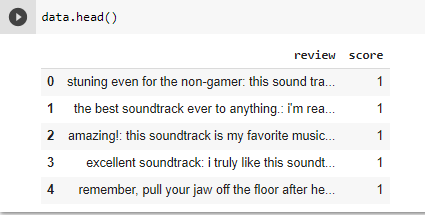
\includegraphics[width=\textwidth]{AI/AmazonDataframe.PNG}
    \caption{\label{amazondataframe}Dataframe voor de Amazon dataset.}
\end{figure}
\FloatBarrier 

\subsection{Twitter dataset}
Het omzetten van de data uit de Twitter dataset verloopt ook gelijkaardig aan de omzetting die gebeurt in hoofdstuk \ref{twitterdatasetomzettenazure}

De data wordt opnieuw opgehaald via Google Drive. De correcte imports worden gedeclareerd en de data wordt ingelezen zoals in figuur \ref{azurestap1twitter}

\subsection{IMDB dataset}
Ook het omzetten van de data uit de IMDB dataset verloopt gelijkaardig aan de omzetting die gebeurt in hoofdstuk \ref{imdbdatasetomzettenazure}.
Na het declareren van de juiste imports, wordt de data opgehaald via Google Drive. De IMDB dataset bevat maar twee kolommen, namelijk de review kolom die de tekst van de review bevat en de sentiment kolom, die 'positive' of 'negative' bevat. 

\section{Data Cleaning}
\label{proofofconceptdatacleaning}
Een tweede stap is het opschonen van de data. In deze stap worden lege velden verwijderd en wordt niet-numerieke data omgezet in numerieke data.

\subsection{Amazon dataset}
Voor de Amazon dataset is er geen cleaning nodig. De data bestaat momenteel uit de review en de score. Er zijn geen overbodige velden of data die moet omgezet worden. Wat natuurlijk wel nog moet gebeuren is de tekst voorbereiden zodat deze op de meest efficiënte manier door het model kan gaan.

Ten eerste is het handig om uit alle reviews de stopwoorden te verwijderen. Deze hebben immers geen impact op de gevoelswaarden van de review. Dit gebeurt via \gls{tokenization}. Meer info hierover kan gevonden worden in sectie \ref{sec:Tokenization}.

\begin{figure}[!htbp]
    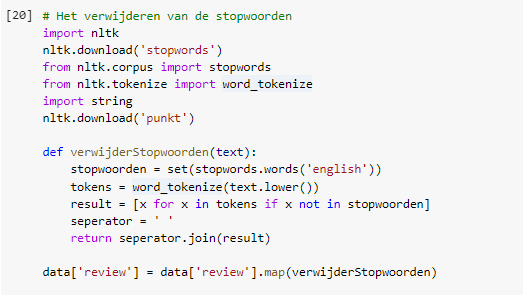
\includegraphics[width=\textwidth]{AI/AmazonTokenization.PNG}
    \caption{\label{amazontokenization}Tokenization voor de Amazon dataset.}
\end{figure}
\FloatBarrier

De data wordt verder verwerkt door er vectors van te maken. Een volledig voorbeeld van de stappen die ondernomen werden is te vinden in bijlage 1.

\subsection{Twitter dataset} 
De Twitter dataset bevat momenteel 15 kolommen, dit is te veel en helemaal niet nodig. De aanmaakdatum, locatie, reden, id,... zijn allemaal velden die niet nodig zijn. Daarom is het de bedoeling om deze tabel om te zetten naar een tabel met enkel de reviews en de scores. 


\begin{figure}[!htbp]
    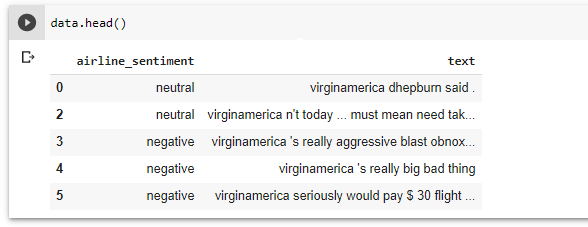
\includegraphics[width=\textwidth]{AI/TwitterData.PNG}
    \caption{\label{twitterdata}Uiteindelijke data voor de Twitter dataset.}
\end{figure}
\FloatBarrier

Voor het verwijderen van de stopwoorden, wordt dezelfde functie als bij de Amazon dataset gebruikt. Deze functie kan gevonden worden in figuur \ref{amazontokenization}. Er is één klein verschil, bij de Twitter dataset moeten de apenstaartjes vooraan de tweets ook verwijderd worden. 

Een tweede omzetting die moet gebeuren, is het omzetten van de woorden 'negatief', 'neutraal' en 'positief' naar 0, 1 en 2. Dit gebeurt aan de hand van onderstaande omzetting:

\begin{figure}[!htbp]
    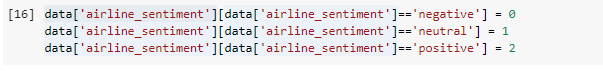
\includegraphics[width=\textwidth]{AI/TwitterOmzetting.PNG}
    \caption{\label{twitteromzetting}Het omzetten van de scores voor de Twitter dataset.}
\end{figure}
\FloatBarrier

\subsection{IMDB dataset}
Voor de IMDB dataset moeten de stopwoorden ook verwijderd worden. Dit is dezelfde functie als in figuur \ref{amazontokenization}. Daarna moeten de woorden 'negative' en 'positive' omgezet worden naar 0 en 1. Deze functie kan men ook vinden in figuur \ref{stap2imdb}. Zoals eerder vermeld, bevat de tekst nog html tags. Deze worden eruit gehaald. Dit gebeurt ook in figuur \ref{stap2imdb}.


\section{Data Exploratie}
\label{proofofconceptdataexploratie}
Dit is een extra toegevoegde stap om eens te gaan kijken wat er juist in de data zit. Dit kan gevisualiseerd worden aan de hand van grafieken, of extra velden. 

\subsection{Amazon dataset}
Om een beter begrip te krijgen van de Amazon dataset, kan men dit op allerlei manieren visualiseren. Momenteel is de Amazon dataset een dataframe. Hierop kan men bijvoorbeeld de functie describe() toepassen. Deze functie toont het aantal rijen data, de gemiddelde score, de \gls{standaardafwijking} (std) en andere gegevens zoals het minimum en het maximum. 

\begin{figure}[!htbp]
    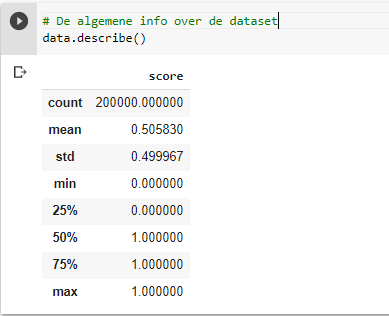
\includegraphics[width=\textwidth]{AI/AmazonDescribe.PNG}
    \caption{\label{amazondescribe}Algemene info over de Amazon dataset.}
\end{figure}
\FloatBarrier 

Hier kan men zien dat er 200.000 rijen data zijn. Het gemiddelde van de data is 0.505, dit betekent dat er een mooie verdeling is tussen positieve en negatieve scores. Het minimum is uiteraard 0 en het maximum is 1. Via de functie data.shape kunnen de dimensies van de data opgevraagd worden. Voor deze dataset is dit (200000,2). De dataset heeft dus 200.000 rijen en twee kolommen. Deze twee kolommen zijn de reviews en de scores. 

Een andere manier om de verdeling tussen de positieve en de negatieve reviews te bekijken, is via een staafdiagram. Deze kan gezien worden in figuur \ref{amazonverdeling} Men kan zien dat er een mooie verdeling is tussen de positieve (oranje balkje) en de negatieve reviews (blauw balkje). Er zijn echter iets meer positieve dan negatieve reviews.

\begin{figure}[!htbp]
    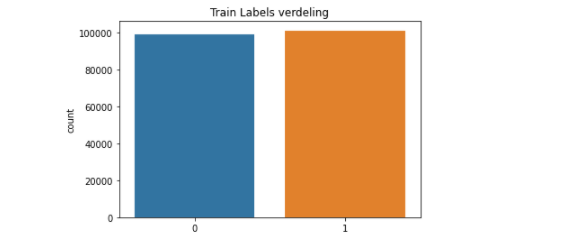
\includegraphics[width=\textwidth]{AI/AmazonVerdeling.PNG}
    \caption{\label{amazonverdeling}Verdeling van de Amazon dataset.}
\end{figure}
\FloatBarrier 

Verder kan ook gekeken worden hoeveel woorden en hoeveel karakters een gemiddelde review bevat en wat de \gls{density} van de reviews is. De density wordt berekend door het aantal woorden door het aantal karakters te delen. Hierdoor geldt het principe dat hoe kleiner de density is, hoe langer de verschillende woorden in de review zijn. 

\begin{figure}[!htbp]
    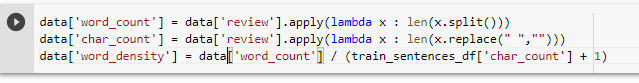
\includegraphics[width=\textwidth]{AI/AmazonExtraVelden.PNG}
    \caption{\label{amazonaantalwoorden}Extra velden voor de Amazon dataset.}
\end{figure}
\FloatBarrier

De resultaten van deze nieuwe kolommen kunnen gevonden worden in figuur \ref{amazondescribe2}.

\begin{figure}[!htbp]
    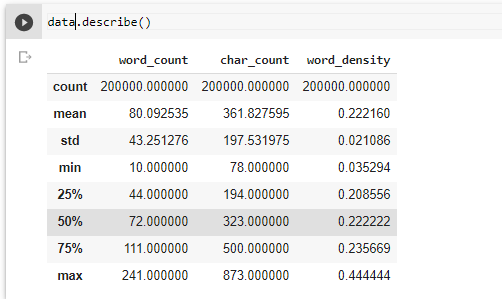
\includegraphics[width=\textwidth]{AI/AmazonDescribe2.PNG}
    \caption{\label{amazondescribe2}Algemene info over de Amazon dataset.}
\end{figure}
\FloatBarrier

Ook hier kan de functie describe op toegepast worden. Het gemiddeld aantal woorden is 80,09, het minimum aantal woorden is 10 en het maximum aantal woorden is 241. Onder de kolom char\_count, kan men zien hoeveel karakters een review gemiddeld bevat. Een review bevat gemiddeld 361.82 karakters, het minimum aantal karakters van een review is 78 en het maximum is 873 karakters. Deze dataset heeft dus een grote variatie aan reviews. Dit kan ook afgeleid worden uit de word\_density, waar het gemiddelde 0.22 is, het minimum 0.035 is en het maximum 0.44 is.

Deze data kan ook in een grafiek gegoten worden.

\begin{figure}[!htbp]
    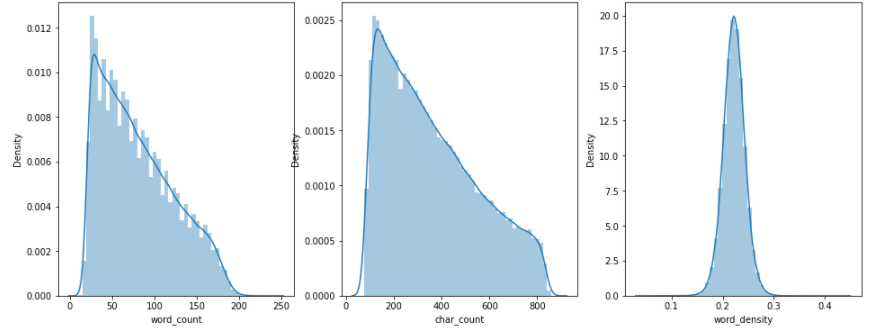
\includegraphics[width=\textwidth]{AI/AmazonExtraGrafiek.PNG}
    \caption{\label{amazongrafiek}Een grafiek over het aantal woorden, karakters en de density van de Amazon dataset.}
\end{figure}
\FloatBarrier


De grafieken zien er alle drie anders uit. Voor het aantal woorden en het aantal karakters springt direct in het oog dat er een grote varieteit is. Dit kan men zien aan de breedte van de grafiek die zich uitstrekt van het minimum tot het maximum. De \gls{density} voor de reviews blijft redelijk dezelfde voor alle reviews. 


\subsection{Twitter dataset}
Voor de Twitter dataset, kan de data ook eens geanalyseerd en gevisualiseerd worden. Na de omzetting kan de score drie betekenissen aannemen. Negatief wordt 0, neutraal wordt 1 en positief wordt 1. Het is dan duidelijk dat het minimum van deze dataset 0 is en het maximum 2 is. Het gemiddelde van de dataset is 0.32. Dit gemiddelde ligt niet zo mooi in het midden als de Amazon dataset. De verdeling van de Twitter dataset is namelijk minder goed. 

Deze verdeling kan ook eens in een grafiek getoond worden.

\begin{figure}[!htbp]
    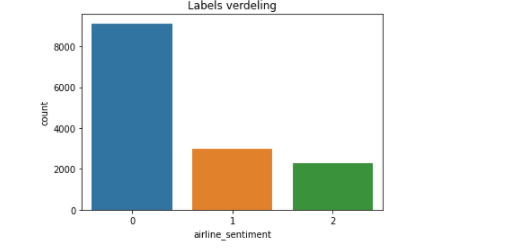
\includegraphics[width=\textwidth]{AI/TwitterVerdeling.PNG}
    \caption{\label{twittergrafiek}Verdeling van de Twitter dataset.}
\end{figure}
\FloatBarrier

Men kan duidelijk zien dat er veel meer negatieve tweets zijn dan neutrale en positieve. Dit kan ervoor zorgen dat de data iets minder betrouwbaar zal zijn. Zoals eerder vermeld zijn tweets ook meestal korter. Dit kan gecontroleerd worden door de functie describe() toe te passen op enkele extra aangemaakte velden.

\begin{figure}[!htbp]
    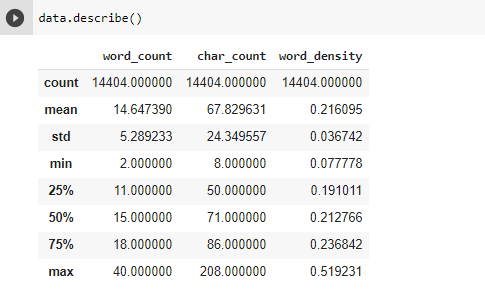
\includegraphics[width=\textwidth]{AI/TwitterExtraData2.PNG}
    \caption{\label{twitterextradata}Extra velden voor de Twitter dataset.}
\end{figure}
\FloatBarrier

Er is een duidelijke tendens zichtbaar. Ten eerste is de omvang van de dataset veel kleiner dan bij de Amazon dataset. De Twitter dataset telt maar 14.404 tweets, terwijl de Amazon dataset 200.000 reviews bevat. Het gemiddeld aantal woorden per tweet is 14. Dit is enorm laag, zeker vergeleken met de Amazon dataset. Het maximum aantal woorden is 40 en het minimum aantal woorden is 2. 
Kan dit een probleem vormen? Is de dataset daarom minder betrouwbaar? Reviews en tweets komen in alle vormen en maten. Een goede AI moet zowel korte als lange reviews/tweets kunnen analyseren. Daarom is het goed om drie compleet verschillende datasets met elkaar te vergelijken. 

Het aantal woorden, karakters en de density kunnen opnieuw in een grafiek geplaatst worden.

\begin{figure}[!htbp]
    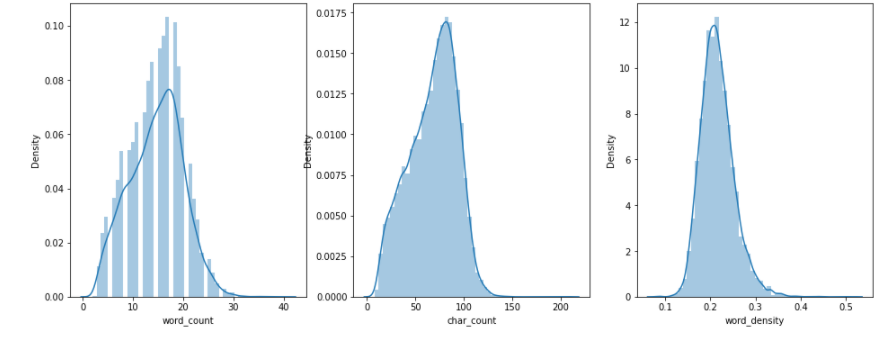
\includegraphics[width=\textwidth]{AI/TwitterExtraGrafiek.PNG}
    \caption{\label{twitterextragrafiek}Een grafiek over het aantal woorden, karakters en de density van de Twitter dataset.}
\end{figure}
\FloatBarrier

\subsection{IMDB dataset}
Dankzij de functie data.describe(), wordt vastgesteld dat de dataset 50.000 reviews bevat. De omvang van de dataset is dan ook (50.000,2).

Om de verdeling van de dataset te beoordelen, wordt dit in een grafiek gegoten. Er blijken evenveel negatieve (blauwe balkje) als positieve (oranje balkje) reviews te zijn. Dit is heel goed, dit betekent dat de IMDB dataset een heel evenwichtige dataset is. 

\begin{figure}[!htbp]
    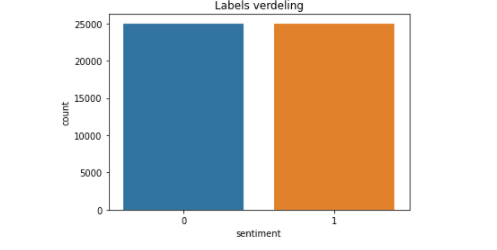
\includegraphics[width=\textwidth]{AI/IMDBVerdeling.PNG}
    \caption{\label{imdbgrafiek}Verdeling van de IMDB dataset.}
\end{figure}
\FloatBarrier

Daarna kunnen opnieuw de extra velden word\_count, char\_count en word\_density toegevoegd worden. 

\begin{figure}[!htbp]
    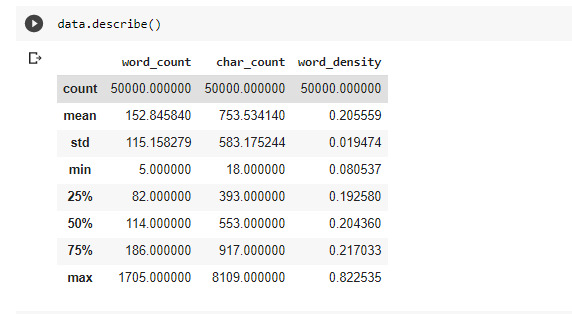
\includegraphics[width=\textwidth]{AI/IMDBExtraData.PNG}
    \caption{\label{imdbextradata}Extra data voor de IMDB dataset.}
\end{figure}
\FloatBarrier

Het gemiddeld aantal woorden is 152.84, met als maximum aantal woorden 1705 en minimum aantal woorden 5. Deze getallen liggen enorm uiteen. Ook het aantal karakters kan afgeleid worden uit bovenstaande tabel. Het gemiddeld aantal karakters is 752, met een maximum van 8109 karakters en een minimum van 18 karakters. De density wordt berekend door het aantal woorden te delen door het aantal karakters. Hoe lager de density, hoe langer de woorden in de review. Het density-gemiddelde is 0.20, het minimum is 0.08 en het maximum is 0.82. Opnieuw liggen deze getallen ver uiteen. Wanneer deze data in een grafiek gegoten wordt, valt dit helemaal niet op.

\begin{figure}[!htbp]
    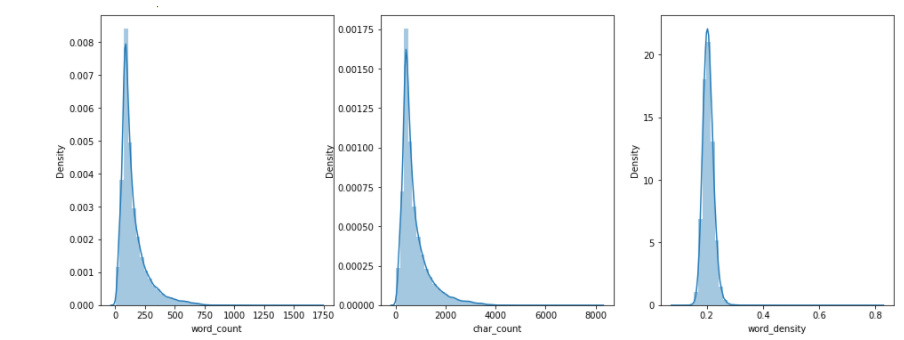
\includegraphics[width=\textwidth]{AI/IMDBExtraGrafiek.PNG}
    \caption{\label{imdbextragrafiek}Een grafiek voor het aantal woorden, karakters en de density van de IMDB dataset.}
\end{figure}
\FloatBarrier

De lengte van de reviews, het aantal karakters en de density ligt voor alle reviews ongeveer bij elkaar. Dit kan geconcludeerd worden uit het feit dat de grafieken niet wijd zijn. Alle data ligt geconcentreerd. De dataset bevat echter wel enkele uitschieters. Daarom dat de maxima en minima zo ver uiteen liggen. 


\section{Opzetten van training dataset en test dataset}
De dataset wordt hier opgesplitst. 70\% van de data wordt training dataset en 30\% van de data wordt test dataset. Dit gebeurt voor alle datasets op dezelfde manier.

\begin{figure}[!htbp]
    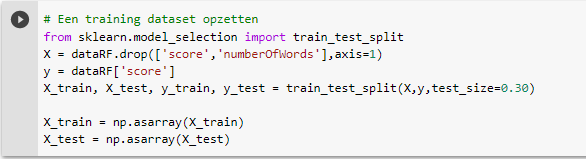
\includegraphics[width=\textwidth]{AI/AmazonValidatie.PNG}
    \caption{\label{amazonopsplitsing}Opsplitsen training en test dataset.}
\end{figure}
\FloatBarrier

\section{Model kiezen}
\label{proofofconceptdatamodel}
Het is enorm moeilijk om het juiste model te kiezen. Een extra laag of epoch kan een groot verschil uitmaken in de nauwkeurigheid van het model. 

\subsection{Model 1}

Een eerste model dat getest wordt, is een \gls{CNN} model: een Convolutional Neural Network. Na enkele testen blijkt dat voor de Amazon dataset 30 epochs meer dan genoeg zijn, terwijl de Twitter dataset betere resultaten toont bij 50 epochs.
\begin{figure}[!htbp]
    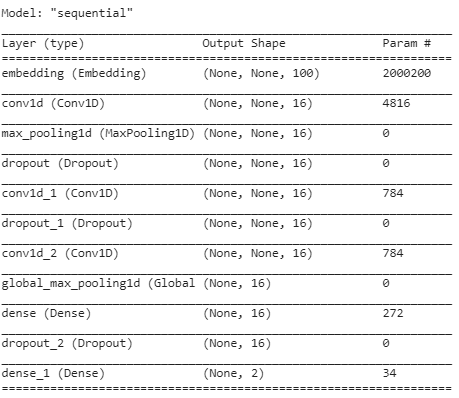
\includegraphics[width=\textwidth]{AI/Model1.PNG}
    \caption{\label{model1}Model 1}
\end{figure}
\FloatBarrier

\begin{figure}[!htbp]
    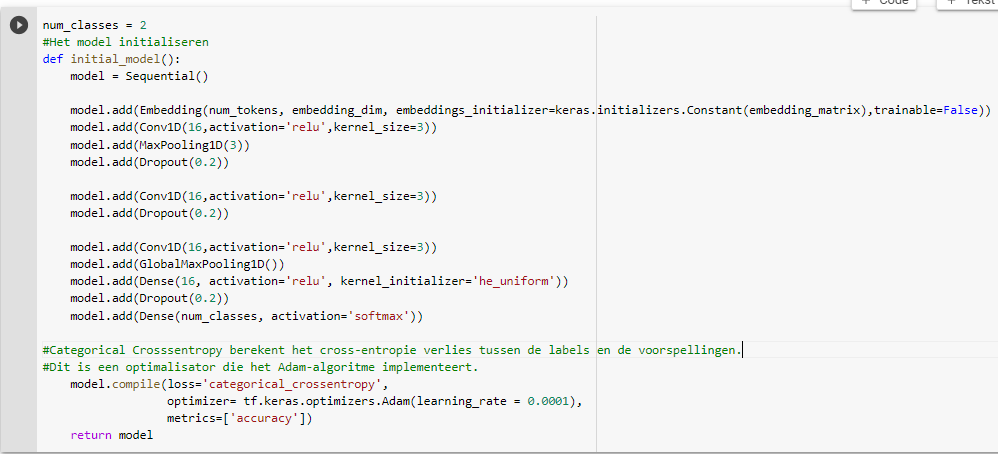
\includegraphics[width=\textwidth]{AI/Model1-2.PNG}
    \caption{\label{model1.2}Model 1}
\end{figure}
\FloatBarrier

Zoals gezien kan worden op figuur \ref{model1}, is het model een sequentieel model. Dit model wordt gebruikt voor een 'stapel' lagen. Elke laag heeft 1 input en 1 output. Daarom wordt hier sequentieel doorgegaan. Het is ook duidelijk dat er een aantal verschillende lagen gebruikt worden. Zowel convolutional layers, dense layers als pooling layers worden hier gebruikt. Meer informatie over deze verschillende lagen kan gevonden worden in sectie \ref{sec:neuralnetworks}. 

Laag 1: Embedding laag: Zet alle positieve getallen, in dit geval de scores om naar vectors. \\
Laag 2: Convolutionele laag met 16 filters en met als activatiefunctie de ReLU, met kernel\_size gelijk aan 3. \\
De kernel size is eigenlijk de grootte van de filter die over de data geschoven wordt. \\
Laag 3: MaxPooling1D: Een pooling layer met lengte 3. In deze laag wordt steeds het maximum berekend van elke feature. Een pooling layer bevindt zich steeds bij een convolutionele laag. \\
Laag 4: Dropout laag met een frequentie van 0.2. Wordt gebruikt om overfitting te vermijden. \\
Laag 5: Convolutionele laag met 16 filters, activatiefunctie ReLU en kernel\_size gelijk aan 3. \\
Laag 6: Dropout laag met een frequentie van 0.2. \\
Laag 7: Convolutionele laag met 16 filters, de ReLU activatiefunctie en kernel\_size 3. \\
Laag 8: GlobalMaxPooling1D laag: een pooling layer die het maximum berekent voor het volledige model. \\
Laag 9: Dense laag: Volledig verbonden laag met 16 filters, een ReLU activatiefunctie en een he\_uniform initializer. \\
Een kernel initializer bepaalt welke verdeling of functie gebruikt moet worden om de gewichten te initialiseren. \\
Laag 10: Dropout laag met een frequentie van 0.2. \\
Laag 11: Dense laag met als output het aantal klassen en activatiefunctie \gls{softmax}. \\
De softmax activatiefunctie wordt gebruikt om de data terug te normaliseren, daarom wordt deze op het einde gebruikt.   

Het duurt even om het model te trainen, maar na een tijdje komen hier resultaten uit. 

Voor de Amazon dataset heeft dit model een nauwkeurigheid van 82\%. Deze worden in een grafiek gestoken zodat men het verloop van de training gedurende de verschillende epochs kan zien. 

\begin{figure}[!htbp]
    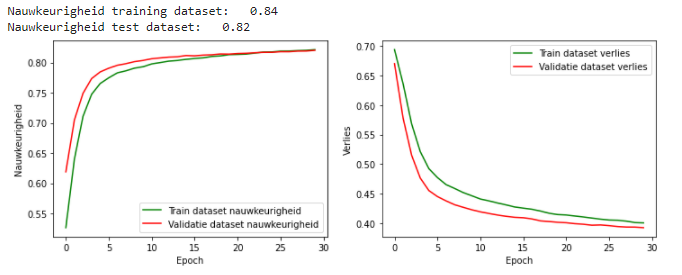
\includegraphics[width=\textwidth]{AI/AmazonResult.PNG}
    \caption{\label{amazonresult}Resultaten Model 1 Amazon dataset.}
\end{figure}
\FloatBarrier

Voor de Twitter dataset heeft dit model een nauwkeurigheid van 75\%
Een belangrijke nota hierbij is dat de Twitter dataset 50 epochs nodig had, terwijl de Amazon dataset 30 epochs nodig had.

Wat is de reden hiervoor?
De Twitter dataset bevat minder data en dus moet de AI aan de hand van minder voorbeelden trainen. Wanneer het aantal epochs verhoogd wordt, doorloopt de AI deze cyclus 50 keer. 
Ook deze resultaten zijn te vinden in een grafiek zoals te zien op figuur \ref{twitterresult}. 

\begin{figure}[!htbp]
    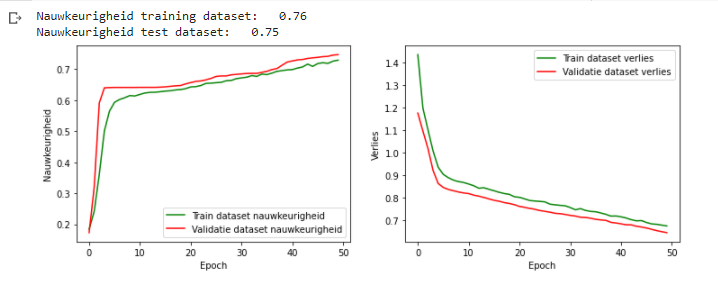
\includegraphics[width=\textwidth]{AI/TwitterResult.PNG}
    \caption{\label{twitterresult}Resultaten Model 1 Twitter dataset.}
\end{figure}
\FloatBarrier

Voor de IMDB dataset heeft dit model een nauwkeurigheid van 72\%.
Ook de IMDB dataset had 50 epochs nodig om een goed resultaat weer te geven. De IMDB dataset bevat ook minder reviews dan de Amazon dataset, dus zijn er meer epochs nodig. Deze resultaten zijn te vinden in de grafiek van figuur \ref{imdbresult}

\begin{figure}[!htbp]
    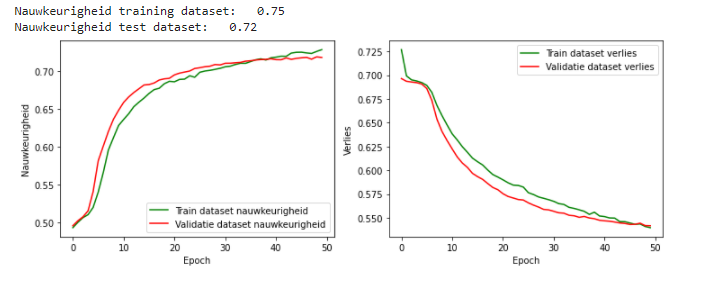
\includegraphics[width=\textwidth]{AI/IMDBResult.PNG}
    \caption{\label{imdbresult}Resultaten Model 1 IMDB dataset.}
\end{figure}
\FloatBarrier

\subsection{Model 2}
In het tweede model werd een andere volgorde van lagen gehanteerd en was het aantal lagen ook minder. Model 2 bleef wel nog steeds een \gls{CNN}. 
Laag 1 is opnieuw een Embedding laag, gevolgd door een Convolutional layer, een GlobalMaxPooling layer en een Dense layer.
Als optimizer wordt opnieuw adam gebruikt.

\begin{figure}[!htbp]
    \includegraphics[width=\textwidth]{Models/Model2OverfittingModel.PNG}
    \caption{\label{overfitting} Model 2.}
\end{figure}
\FloatBarrier

Bij dit model bleek er echter overfitting te zijn. Dit kan men zien doordat er een groot verschil is in de grafiek tussen de training en test dataset nauwkeurigheid.

\begin{figure}[!htbp]
    \includegraphics[width=\textwidth]{Models/Model2AmazonResult.PNG}
    \caption{\label{overfittingresult} Resultaten Model 2 Amazon dataset: overfitting.}
\end{figure}
\FloatBarrier

Daarom was het verstandig om enkele \gls{dropoutlaag} toe te voegen. Dropout lagen vermijden overfitting. Model 2 zag er daardoor als volgt uit:

\begin{figure}[!htbp]
    \includegraphics[width=\textwidth]{Models/Model2.PNG}
    \caption{\label{model2.1} Model 2.1.}
\end{figure}
\FloatBarrier

\begin{figure}[!htbp]
    \includegraphics[width=\textwidth]{Models/Model2Summary.PNG}
    \caption{\label{model2.1summary} Model 2.1.}
\end{figure}
\FloatBarrier


Dit model werd dan op de drie datasets toegepast. Voor de eerste dataset, de Amazon dataset, behaalde dit model een nauwkeurigheid van 82\% Op de test dataset.

\begin{figure}[!htbp]
    \includegraphics[width=\textwidth]{Models/Model2-1AmazonResult.PNG}
    \caption{\label{amazonresult2}Resultaten Model 2 Amazon dataset.}
\end{figure}
\FloatBarrier

Model 2 behaalde voor de Twitter dataset een nauwkeurigheid van 78\%.

\begin{figure}[!htbp]
    \includegraphics[width=\textwidth]{Models/Model2-1TwitterResult.PNG}
    \caption{\label{twitterresult2}Resultaten Model 2 Twitter dataset.}
\end{figure}
\FloatBarrier

Voor de IMDB dataset werd een nauwkeurigheid van 73\% behaald.

\begin{figure}[!htbp]
    \includegraphics[width=\textwidth]{Models/Model2-1IMDBResult.PNG}
    \caption{\label{imdbresult2}Resultaten Model 2 IMDB dataset.}
\end{figure}
\FloatBarrier

\subsection{Model 3}

Model 3 is opnieuw een Sequentieel model met als eerste laag een Embeddingslaag zodat de embeddings matrix gemakkelijk kan toegevoegd worden.

\begin{figure}[!htbp]
    \includegraphics[width=\textwidth]{Models/Model3Amazon.PNG}
    \caption{\label{model3}Model 3.}
\end{figure}
\FloatBarrier

Laag 2 bestaat uit een LSTM laag met 2 parameters. LSTM staat voor Long short-term memory en is een voorbeeld van een \gls{RNN}: Recurrent Neural Network. LSTM bevat feedbackverbindingen waarbij bij elke stap beslist zal worden welke data er bewaard wordt en welke vergeten wordt. 
\begin{figure}[!htbp]
    \includegraphics[width=\textwidth]{Models/Model3Amazon2.PNG}
    \caption{\label{model3.2}Model 3.}
\end{figure}
\FloatBarrier

Dit model werd op drie datasets toegepast. Voor de Amazon dataset had dit model een nauwkeurigheid van 82\%

\begin{figure}[!htbp]
    \includegraphics[width=\textwidth]{Models/Model3AmazonResult.PNG}
    \caption{\label{model3amazon}Resultaten Model 3 Amazon dataset.}
\end{figure}
\FloatBarrier

Model 3 leverde voor de Twitter dataset een nauwkeurigheid van 76\% op.

\begin{figure}[!htbp]
    \includegraphics[width=\textwidth]{Models/Model3TwitterResult.PNG}
    \caption{\label{model3twitter}Resultaten Model 3 Twitter dataset.}
\end{figure}
\FloatBarrier

Ten slotte, voor de IMDB dataset werd er een nauwkeurigheid van 72\% geteld.

\begin{figure}[!htbp]
    \includegraphics[width=\textwidth]{Models/Model3IMDBResult.PNG}
    \caption{\label{model3imdb}Resultaten Model 3 IMDB dataset.}
\end{figure}
\FloatBarrier

\subsection{Model 4}
Een laatste model dat getest werd, is model 4. Model 4 is opnieuw een Sequentieel model met als eerste laag een embedding laag. Naast het feit dat er opnieuw een LSTM (Long short-term memory) laag gebruikt wordt, bevindt deze zich nu in een Bidirectionele laag. Deze laag verbindt twee verborgen lagen die uit een tegengestelde richting komen met eenzelfde output. Het voordeel hiervan is dat deze outputlaag tegelijk de informatie uit het verleden en uit de toekomst bevat. Dit model is opnieuw een RNN (Recurrent Neural Network). Omdat dit in een bidirectionele laag zit, wordt dit ook een BRNN (Bidirectional Recurrent Neural Network) genoemd.

Na deze laag komen er enkele bekende lagen. Een Dense laag met als activatiefunctie ReLU staat op de derde laag. De vierde laag is een Dropoutlaag met 0.50 dropout frequentie. Dit wordt opnieuw gebruikt om overfitting te vermijden. Laag 5 is opnieuw een Dense laag, maar met als activatiefunctie de softmax.

\begin{figure}[!htbp]
    \includegraphics[width=\textwidth]{Models/Model4.PNG}
    \caption{\label{model4}Model 4.}
\end{figure}
\FloatBarrier

De drie datasets werden opnieuw door dit model getraind. 30 epochs bleek hier de beste resultaten op te leveren. Voor de Amazond dataset leverde model 4 een nauwkeurigheid van 85\% op.

\begin{figure}[!htbp]
    \includegraphics[width=\textwidth]{Models/Model4AmazonResult.PNG}
    \caption{\label{model4amazon}Resultaten Model 4 Amazon dataset.}
\end{figure}
\FloatBarrier

Voor de Twitter dataset behaalde model 4 een nauwkeurigheid van 80\%.

\begin{figure}[!htbp]
    \includegraphics[width=\textwidth]{Models/Model4TwitterResult.PNG}
    \caption{\label{model4twitter}Resultaten Model 4 Twitter dataset.}
\end{figure}
\FloatBarrier

Ten slotte behaalde model 4 voor de IMDB dataset een nauwkeurigheid van 75\%.

\begin{figure}[!htbp]
    \includegraphics[width=\textwidth]{Models/Model4IMDBResult.PNG}
    \caption{\label{model4imdb}Resultaten Model 4 IMDB dataset.}
\end{figure}
\FloatBarrier

\section{Samenvatting}
Om de resultaten van alle modellen te kunnen vergelijken, staan deze opgesomd in onderstaande tabel (zie tabel \ref{tab:samenvattingproofofconcept}). Men kan zien dat elk model redelijk goede gemiddelde scores behaalde. Uit de tabel 'Totaal' leidt men af dat model 4 de beste resultaten behaalde, zowel op de Amazon dataset, de Twitter dataset als op de IMDB dataset.

Ondanks dat de resultaten van model 2 redelijk goed waren, treedt er hier en daar wat overfitting op. Model 2 is daarom niet het juiste model om reviews te kunnen analyseren. Model 4 blijft het beste model om NLP toe te passen.


\begin{table}[htb]
    \centering
    \begin{tabular}{@{}llllll@{}}
        \toprule
        & Type Neural Network & Amazon & Twitter & IMDB & Totaal \\ \midrule
        Model 1 & \gls{CNN}                 & 82\%                  & 75\%                   & 72\%                & 76.3\% \\
        Model 2 & CNN                 & 82\%                  & 78\%                   & 73\%                & 77.6\% \\
        Model 3 & \gls{RNN}                 & 82\%                  & 76\%                   & 72\%                & 76.6\% \\
        Model 4 & RNN                 & 85\%                  & 80\%                   & 75\%                & 80\%   \\ \bottomrule
    \end{tabular}
    \caption{Samenvatting resultaten proof of concept}
    \label{tab:samenvattingproofofconcept}
\end{table}
\FloatBarrier


% Voeg hier je eigen hoofdstukken toe die de ``corpus'' van je bachelorproef
% vormen. De structuur en titels hangen af van je eigen onderzoek. Je kan bv.
% elke fase in je onderzoek in een apart hoofdstuk bespreken.

%\input{...}
%\input{...}
%...

%%=============================================================================
%% Conclusie
%%=============================================================================

\chapter{Conclusie}
\label{ch:conclusie}

% TODO: Trek een duidelijke conclusie, in de vorm van een antwoord op de
% onderzoeksvra(a)g(en). Wat was jouw bijdrage aan het onderzoeksdomein en
% hoe biedt dit meerwaarde aan het vakgebied/doelgroep? 
% Reflecteer kritisch over het resultaat. In Engelse teksten wordt deze sectie
% ``Discussion'' genoemd. Had je deze uitkomst verwacht? Zijn er zaken die nog
% niet duidelijk zijn?
% Heeft het onderzoek geleid tot nieuwe vragen die uitnodigen tot verder 
%onderzoek?

De onderzoeksvraag van deze bachelorproef luidde als volgt: `In welke mate kunnen AI's getraind worden om menselijke gevoelswaarden te herkennen in teksten?'. Deze vraag werd beantwoord door ten eerste twee externe tools zoals de Azure Text Analytics API en Google Cloud Platform te onderzoeken in hoofdstuk \ref{ch:methodologie}. Ten tweede werd ook een proof of concept gemaakt om op deze vraag te kunnen beantwoorden in hoofdstuk \ref{ch:proof-of-concept}. Deze bachelorproef onderzocht of AI sentimentele data kan halen uit reviews. Daarom werden er drie datasets gebruikt. Twee van deze dataset bevatten reviews en/of klachten die van de website zelf gehaald werden. Eén dataset bevatte tweets met reviews over vliegtuigmaatschappijen. Dit werd gedaan om variatie te creëren en zo een beter beeld te krijgen van de resultaten.

In welke mate kunnen AI's getraind worden om menselijke gevoelswaarden te herkennen in teksten? Natural Language Processing en Sentiment Analysis staan al heel ver. Er zijn verschillende tools en modellen die aan het vooraf bepaalde 80\% succespercentage voldoen. Google Cloud Platform bleek echter de beste resultaten te behalen.

Er waren ook een aantal deelvragen gedefinieerd. Deze zullen zo goed mogelijk beantwoord worden.

\section{Hoe ver staan Natural Language Processing en Sentiment Analysis al?}
\label{sec:hoever}
Op deze vraag kan duidelijk geantwoord worden dat NLP en Sentiment Analysis al heel ver staan. Zowel voor de externe tools, als voor de modellen werden er redelijk goede resultaten behaald op de drie datasets.
Voor alle modellen en externe tools werd ten minste een score van 75\% behaald. Dit betekent dat NLP en Sentiment Analysis al enorm gevorderd zijn.
In figuur \ref{fig:modellen} staan de modellen die in de proof of concept besproken werden. Het valt op dat alle modellen een redelijk goede score behaald hebben. Echter was model vier, wat een RNN (Recurrent Neural Netwerk) was, het beste model. Dit model voldeed wel aan de vooraf gedefinieerde 80\%.

\begin{figure}[!htbp]
    \includegraphics[width=\textwidth]{Grafieken/Modellen.PNG}
    \caption{\label{fig:modellen}Resultaten van alle modellen.}
\end{figure}
\FloatBarrier

In figuur \ref{fig:methodes} staat het beste model van de proof of concept in vergelijking met de twee externe methodes. Hier valt op dat Google Cloud Platform de beste gemiddelde resultaten opleverde. 

\begin{figure}[!htbp]
    \includegraphics[width=\textwidth]{Grafieken/methodes.PNG}
    \caption{\label{fig:methodes}Resultaten van alle methodes.}
\end{figure}
\FloatBarrier

Hieruit kan geconcludeerd worden dat NLP al heel ver staat, maar dat er nog ruimte is voor verbetering.

\section{Kunnen AI's bepaalde gevoelswaarden al begrijpen?}
\label{sec:gevoelswaarden}
Ja. Het is duidelijk dat AI's gemakkelijk het verschil tussen positieve, neutrale en negatieve reviews kunnen analyseren. Door de goede resultaten op de drie datasets, kan geconcludeerd worden dat NLP en AI's goed gevoelswaarden kunnen herkennen.

\section{Kunnen bedrijven Sentiment Analysis en Opinion Mining gebruiken bij het analyseren van hun reviews?}
\label{sec:reviews}
Het is enorm handig voor bedrijven om met de klant te kunnen communiceren aan de hand van gevoelswaarden die uit hun reviews afgeleid worden.
Het vooraf gedefinieerde succespercentage van 80\% werd bereikt. Daaruit kan besloten worden dat bedrijven dit zeker in de praktijk kunnen toepassen. Dit verhoogt immers de verstandshouding tussen het bedrijf en de klant.

\section{Verder Onderzoek}
\label{sec:verderonderzoek}
Natuurlijk is verder onderzoek nog vereist. Ten eerste zou het interessant zijn om verder onderzoek te doen naar hoe Artificiële Intelligentie gepast kan reageren op een review. Nu het duidelijk is dat AI gevoelswaarden uit een review kan afleiden, is verder onderzoek naar hoe men hierop reageert belangrijk. Verder kan er ook onderzoek gedaan worden naar modellen of methodes die een succespercentage van 90\% kunnen bereiken. Dit betekent meer zekerheid voor de bedrijven dat de AI juist reageert op de wensen van de klant.



%%=============================================================================
%% Bijlagen
%%=============================================================================

\appendix
\renewcommand{\chaptername}{Appendix}

%%---------- Onderzoeksvoorstel -----------------------------------------------

\chapter{Onderzoeksvoorstel}

Het onderwerp van deze bachelorproef is gebaseerd op een onderzoeksvoorstel dat vooraf werd beoordeeld door de promotor. Dat voorstel is opgenomen in deze bijlage.

% Verwijzing naar het bestand met de inhoud van het onderzoeksvoorstel
%---------- Inleiding ---------------------------------------------------------

\section{Introductie} % The \section*{} command stops section numbering
\label{sec:introductie}

Artificiële intelligentie heeft de afgelopen jaren al heel wat vooruitgang geboekt. Ook op het vlak van vertalingen zien we veel tools opduiken zoals Google Translate en DeepL die een redelijk goede vertaling aan de gebruiker kunnen aanbieden. Vaak volstaan deze vertalingen niet omdat Artificiële Intelligentie geen emotionele gevoelswaarden of culturele aspecten, zoals beleefdheidsvormen, kan verstaan of vertalen. De betekenis of zelfs context van veel zinnen gaat zo verloren. Maar zou het niet handig zijn moest een AI gevoelswaarden kunnen afleiden uit een tekst? Denk maar aan bedrijven waarvoor de klanten recensies kunnen schrijven. De AI zou dan aan de hand van detectiesoftware bepaalde gevoelswaarden kunnen herkennen. Het bedrijf in kwestie kan dan inspelen op de gevoelens van elke afzonderlijke klant, wat enorm veel voordelen met zich oplevert.
Een voorbeeld hiervan: een klant laat een boze, ontevreden recensie achter. De AI detecteert dat dit een boze recensie is, en speelt hierop in met een verontschuldigend antwoord en misschien zelfs een compensatie.  
In deze bachelorproef zal dit thema onderzocht worden: kunnen AI’s getraind worden om gevoelswaarden in een tekst te begrijpen en hiernaar correct te handelen? Daarbij worden volgende vragen onderzocht:

\begin{itemize}
  \item Hoe ver staan Natural Language Processing en Sentiment Analysis al?
  \item Kunnen AI's bepaalde gevoelswaarden al begrijpen?
  \item In welke mate kunnen AI's deze gevoelswaarden begrijpen?
  \item Kunnen bedrijven Sentiment Analysis en Opinion Mining gebruiken bij het analyseren van hun reviews?
\end{itemize}

%---------- Stand van zaken ---------------------------------------------------

\section{State-of-the-art}
\label{sec:state-of-the-art}

Artificiële Intelligentie heeft al heel wat vorderingen gemaakt op het vlak van het analyseren van teksten. Maar deze analyses verstaan nooit de gevoelswaarde die de auteur in de tekst probeert te brengen. 
Het vakgebied van artificiële intelligentie dat hierover handelt, heet Natural Language Processing of NLP. NLP houdt zich vooral bezig met de interactie tussen computers en menselijke taal. NLP onderzoekt of een AI in staat is om de inhoud van een tekst te begrijpen. De uitdaging is hier om ook gevoelens uit deze teksten te halen.~\autocite{Knight1997}
Een vaak gebruikte techniek bij NLP is sentiment analysis, ook bekend als opinion mining. Deze techniek bepaalt of data een positieve, negatieve of neutrale connotatie heeft. ~\autocite{MonkeyLearn2020}
Er zijn al een aantal onderzoeken gedaan naar de mogelijkheid om AI’s de kennis over gevoelswaarden te geven. ~\autocite{ChewYean2015} Microsoft heeft zo een Tekst Analytics API ontworpen. ''De Text Analytics API is een cloud-gebaseerde dienst die Natural Language Processing (NLP) functies biedt voor text mining en tekstanalyse, waaronder: sentiment analysis, opinion mining,key phrase extraction, language detection en named entity recognition.'' ~\autocite{Microsoft2020} Er werd hiervoor een  Text Analytics Library ontworpen. Hierbij kan men over een zin zeggen of deze een negatieve, neutrale of positieve connotatie heeft. Dit onderzoek zal verder uitgewerkt worden in de bachelorproef.
Verder zal er geprobeerd worden om zelf een dataset te trainen en de hoogst mogelijke accuracy proberen te halen met behulp van een al eerder aangemaakte dataset van een aantal reviews ~\autocite{Minqing2004}. 


% Voor literatuurverwijzingen zijn er twee belangrijke commando's:
% \autocite{KEY} => (Auteur, jaartal) Gebruik dit als de naam van de auteur
%   geen onderdeel is van de zin.
% \textcite{KEY} => Auteur (jaartal)  Gebruik dit als de auteursnaam wel een
%   functie heeft in de zin (bv. ``Uit onderzoek door Doll & Hill (1954) bleek
%   ...'')


%---------- Methodologie ------------------------------------------------------
\section{Methodologie}
\label{sec:methodologie}

Om uit te testen hoe ver AI al staat met het analyseren van een tekst en de gevoelens van deze tekst, zal de hierboven vermelde Microsoft library getest worden in Visual Studio. Er zullen een honderdtal zinnen weergegeven worden, en op basis van deze zinnen zal er gekeken worden hoe goed deze tool is om recensies en opmerkingen te analyseren. Zinnen die goed geanalyseerd worden zullen een 1 toegekend krijgen, terwijl zinnen die slecht geanalyseerd worden een 0 krijgen. Onder 'goed' verstaan we een positieve zin die beoordeeld wordt als positief, een negatieve zin als negatief en een neutrale zin als neutraal. 
In dit onderzoek zal de data van een al bestaande dataset getraind worden om te kijken of AI al ver genoeg staat zodat bedrijven hun recensies zouden kunnen laten analyseren. Verder onderzoek over welke dataset zal gebruikt worden is nog nodig.


%---------- Verwachte resultaten ----------------------------------------------
\section{Verwachte resultaten}
\label{sec:verwachte_resultaten}

Wat er verwacht wordt van de resultaten na de testen uitgevoerd te hebben, is dat Artificiële Intelligentie al ver staat, maar dat het detecteren van emoties in teksten nog niet perfect is. Er zijn al heel wat studies en experimenten uitgevoerd over dit onderwerp, maar er zijn enorm veel nuances aan een taal, waardoor verwacht wordt dat de huidige tools de tekst nog niet perfect kunnen evalueren. Voor het evalueren van de gevoelswaarden van recensies voor bedrijven wordt er verwacht dat de huidige tools en de huidige kennis wel genoeg zijn.
Bij de Microsoft Library worden redelijk goede resultaten verwacht. Er wordt verwacht dat 85-90 procent van de zinnen juist geanalyseerd zal worden. De Microsoft Library geeft enkel aan of een zin een positieve, negatieve of neutrale connotatie heeft. Bij het trainen van een al eerder gedefineerde dataset, met eigen geschreven training en testing worden er iets minder goede resultaten verwacht. We verwachten hier dat 75-80 procent van de zinnen correct geanalyseerd zal worden.



%---------- Verwachte conclusies ----------------------------------------------
\section{Verwachte conclusies}
\label{sec:verwachte_conclusies}

De conclusie die verwacht wordt is de volgende: Artificiële Intelligentie is wel klaar om door bedrijven toegepast te worden om het gevoel van hun klanten in reviews of teksten te herkennen en hier gepast op te handelen. Het is echter heel moeilijk voor AI’s om het menselijk denken en handelen in een dataset te plaatsen en deze te analyseren. Ondanks dat AI nog niet in staat is om alle zinnen correct te analyseren, staat AI wel al ver genoeg om opinion mining in het echte leven bij bedrijven te gebruiken.



%%---------- Andere bijlagen --------------------------------------------------
\chapter{Verklarende woordenlijst}
% TODO: Voeg hier eventuele andere bijlagen toe
%%=============================================================================
%% Verklarende Woordenlijst
%%=============================================================================


Dit is een lijst van alle belangrijke termen die in deze bachelorproef worden aangehaald. Wanneer de lezer tijdens het lezen een opfrisser wil van een bepaalde term, kan hij of zij hier terecht.

\printglossary[title=Glossary, toctitle=List of terms]

    

\chapter{Bijlage 1: Amazon Model 1}
\includepdf[pages=-,offset=0 -0]{bijlagen/AmazonModel1.pdf}
\chapter{Bijlage 2: Twitter Model 1}
\includepdf[pages=-,offset=0 -0]{bijlagen/TwitterModel1.pdf}
\clearpage

%%---------- Referentielijst --------------------------------------------------

\printbibliography[heading=bibintoc]

\end{document}
